\documentclass[ %
    11pt, %
    a4paper, %
    BCOR=12mm, %
    DIV=12, %
    headsepline=true, %
    parskip=half, %
    %draft=true, %
]{article}

\usepackage[utf8]{inputenc}
\usepackage[T1]{fontenc}
\usepackage{lmodern}
\usepackage{braket}
%%englisches Protokoll
%\usepackage[british,UKenglish,USenglish,english,american]{babel}
% %
%%deutsches Protokoll
\usepackage[ngerman]{babel}
% %
\usepackage{amssymb,amsmath,setspace}
\usepackage{engrec}
\usepackage{enumerate}
\usepackage{empheq}
\usepackage{picins}
\usepackage{floatflt}
\usepackage{graphicx}
\usepackage{color}
\usepackage{natbib}
\usepackage{pdfpages}
\usepackage{hyperref}
\graphicspath{{Bilder/}}%% Allgemeine Bilder
\usepackage[paper=a4paper,left=25mm,right=25mm,top=25mm,bottom=25mm]{geometry}

\begin{document}


\begin{titlepage}

\begin{center}




\includegraphics[width=0.3\textwidth]{Bilder/logo}\\[1.2cm]    

\textsc{\LARGE Albert-Ludwigs-Universit\"at Freiburg}\\[1.75cm]

\textsc{\Large Physikalisches Fortgeschrittenen-Praktikum I}\\[0.75cm]



\newcommand{\HRule}{\rule{\linewidth}{0.5mm}}
\HRule \\[0.5cm]
{ \huge \bfseries Szintillationszähler}\\[0.5cm]

\HRule \\[1.75cm]


\begin{minipage}{0.4\textwidth}
\begin{flushleft} \large
\emph{Studenten:}\\
Daniel \textsc{Uhl}\\ \setlength{\parindent}{1.25cm} \& 
\setlength{\parindent}{0cm} \\ Jan P\'eter \textsc{Szabados} 
\end{flushleft}
\end{minipage}
\hfill
\begin{minipage}{0.4\textwidth}
\begin{flushright} \large
\emph{Tutor:} \\
Matthias \textsc{Gorzellik}\\
\end{flushright}
\end{minipage}

\vfill


{\large \today}

\end{center}

\end{titlepage}

\pagenumbering{Roman}

\tableofcontents
\newpage
\pagenumbering{arabic}
\section{Theoretische Grundlagen}

\newcommand{\VG}{V_{\mathbf{G}}}
\newcommand{\G}{\mathbf{G}}
\newcommand{\g}{\mathbf{g}}
\newcommand{\R}{\mathbf{r}}
\newcommand{\K}{\mathbf{k}}
\newcommand{\A}{\mathbf{a}}
\newcommand{\ex}{\mathbf{e}^}
\subsection{Theorie des Quantentunnelns}
\textit{Quantentunneln}, oder kurz \textit{Tunneln} 
bezeichnet das quantenmechanische Phänomen, wenn 
die Durchtrittswahrscheinlichkeit eines Teilchens
durch eine Potenzialbarriere nicht null ist, selbst wenn die Energie
des Teilchens geringer ist als das Potenzial selbst ($E < V$), was
in der klassischen Mechanik nicht möglich wäre. Dies
spielt eine wichtige Rolle bei
vielen Phänomenen in Natur und Technik,
beispielsweise bei der Kernfusion der Sonne, bei der Diode und
daher auch beim Transistor und somit bei der Funktionionsweise
eines Computers an sich, aber auch beim Quantencomputer oder
eben in unserem Fall beim RTM. Das Phänomen des Quantentunnelns
wurde Anfang des 20ten Jahrhunderts mit der Entdeckung der 
Quantenmechanik postuliert und Mitte des Jahrhunderts bestätigt.
\subsection{Mathematische Herleitung von Quantentunneln}
In den folgenden Ausführungen werden Kenntnisse der Quantenmechanik
vorrausgesetzt. Betrachten wir zunächst die Zeitunabhängige
Schrödingergleichung für ein Teilchen in einer Dimension:
\begin{align}
\left [ \frac{-\hbar^2}{2m}\partial_x^2 + V(x) \right ]\psi(x) = E\psi(x) \\ 
\Leftrightarrow \left [ \frac{-\hbar^2}{2m}\partial_x^2 \right ]\psi(x) = \left [E-V(x) \right ]\psi(x) 
\end{align}
Im Spezialfall wenn $V(x)$ konstant ist, können wir die Gleichung
sofort mit planaren Wellen lösen:
\begin{align}
    k^2 = \frac{2m}{\hbar^2}(V-E)\\
    \psi(x) \sim \exp(ikx) 
\end{align}
\subsubsection{Rechteckspotenzial}
Nehmen wir nun an, das Potenzial ist gegeben durch:
\begin{equation}
    V(x) = V_0 \left [ \Theta(x) - \Theta(x-a) \right ] 
\end{equation}
Wobei $\Theta(x)$ die Heavisidefunktion ist und $V_0 > E$.
Die Barriere teilt den Raum nun in drei Teile, $x<0$, $0\leqslant x\leqslant a$ und $a<x$.
In jedem dieser Teile ist das Potenzial konstant, somit können wir für jeden Teil eine
obere Lösung ansetzen \cite{wolfgang2010experimentalphysik},
\cite{landau1991quantenmechanik}:
\begin{align}
    \psi_I(x)    &= A_r \exp(ik_0x) + A_l  \exp(-ik_0x) \mbox{ for } x<0\\
    \psi_{II}(x) &= B_r \exp(ik_1x) + B_l  \exp(-ik_1x) \mbox{ for } 0 \leqslant x \leqslant a\\
    \psi_{III}(x)&= C_r \exp(ik_0x) + C_l  \exp(-ik_0x) \mbox{ for } x>0
\end{align}
Für $E>V_0$ gilt nun:
\begin{align}
    k_0 &= \frac{\sqrt{2mE}}{\hbar}\\
    k_1 &= \frac{\sqrt{2m(E-V_0)}}{\hbar}
\end{align}
Die Koeffizienten A,B und C lassen sich nun mit den Randbedingungen
für die Stetigkeit lösen:
\begin{align}
    \psi_I(0)&\overset{!}{=} \psi_{II}(0)\\
    (\partial_x\psi_I)(0)&\overset{!}{=} (\partial_x\psi_{II})(0)\\
    \psi_{II}(a)&\overset{!}{=} \psi_{III}(a)\\
    (\partial_x\psi_{II})(a)&\overset{!}{=} (\partial_x\psi_{III})(a)
\end{align}
Dies ergibt nach einsetzen der Lösungen für die Wellenfunktionen:
\begin{align}
  A_r + A_l &= B_r + B_l \\
  ik_0(A_r-A_l) &= ik_1(B_r-B_l)\\
  B_r\exp(iak_1)+B_l\exp(-iak_1)&=C_r \exp(iak_0)+C_l\exp(-iak_0)\\
  ik_1(B_r\exp(iak_1) - B_l\exp(-iak_1))&=ik_0(C_r\exp(iak_0)-C_l\exp(-iak_0))
\end{align}
Dies sind 6 freie Parameter für 4 Gleichungen, also können wir zwei 
Paramter festsetzen. Wir setzen $A_r =1$ (Skalierung nach der einlaufenden
Welle) und $C_l = 0$, das bedeutet, dass keine Welle von rechts dazukommt,
sondern alles von der einlaufenden Welle $A_r$ abhängt. Des weiteren
benennen wir $A_l=r$ für Reflexion, und $C_r=t$ für Transmission. Nun
lassen sich die Gleichungen nach diesen Koeffizienten auflösen:
\begin{align}
    t &= \frac{4k_0k_1\exp(-ia(k_0-k_1))}{(k_0+k_1)^2 - \exp(2iak_1)(k_0-k_1)^2}\\
    r &= \frac{(k_0^2 - k_1^2)\sin(ak_1)}{2ik_0k_1\cos(ak_1)+(k_0^2+k_1^2)\sin(ak_1)}
\end{align}
Nun lässt sich mit diesen Ausdrücken die Übergangswahrscheinlichkeit durch die 
Barriere berechnen:
\begin{align}
    T = \left | t \right |^2 = \frac{1}{1 + \frac{V_0^2 \sinh^2(k_1a)}{4E(V_0-E)}}
    \label{eq:T1}
\end{align}
Wenn das Potenzial kleiner ist als die Energie, läuft die Rechung analog
(wobei $k_1 = \frac{\sqrt{2m(V_0-E)}}{\hbar}$) und wir erhalten:
\begin{align}
    T = \left | t \right |^2 = \frac{1}{1 - \frac{V_0^2 \sin^2(k_1a)}{4E(V_0-E)}}
    \label{eq:T2}
\end{align}

\begin{figure}

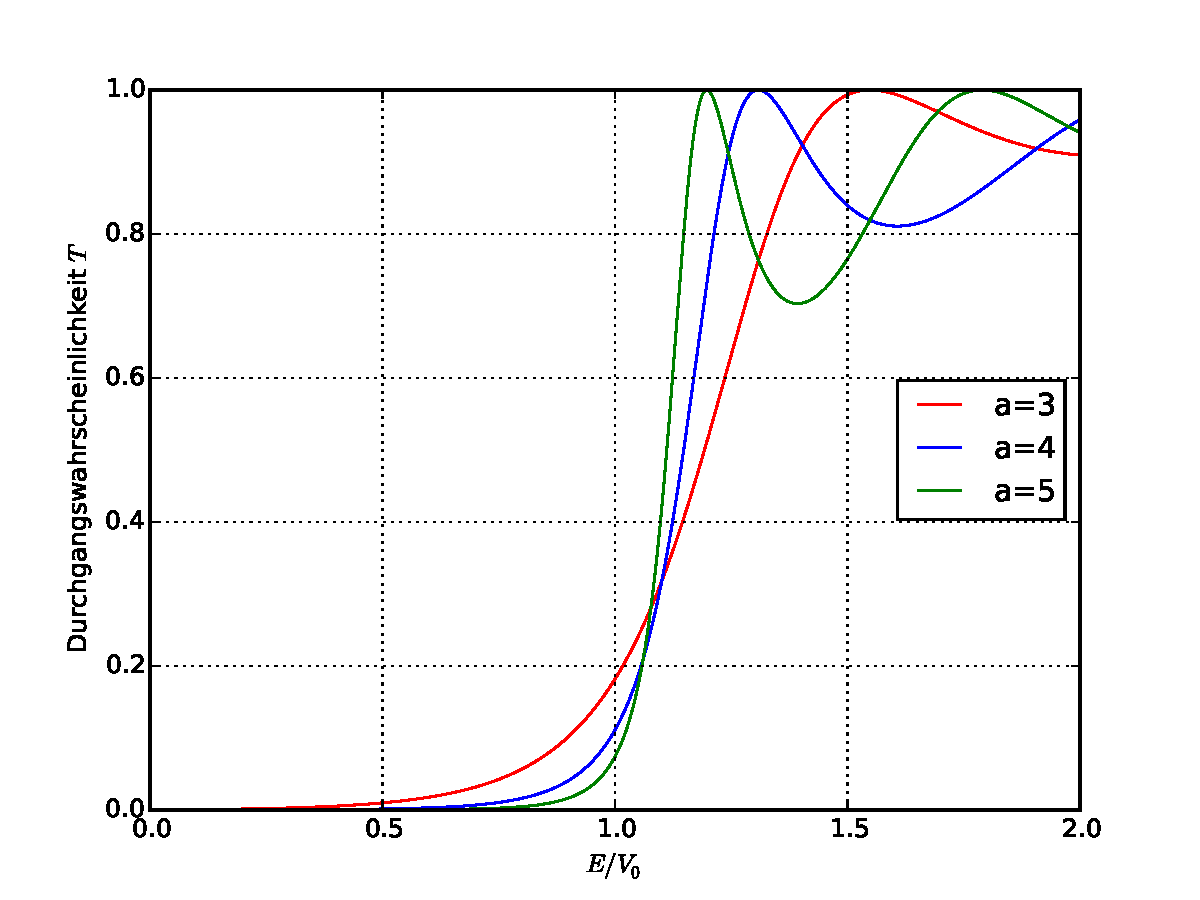
\includegraphics[width=14cm]{pics/tunnel1}
\caption{Transmissionswahrscheinlichkeit nach Gleichung~\ref{eq:T1} und Gleichung~\ref{eq:T2}
bei verschiedenen Breiten des Potenzials $a$ (obdA wurde hier $\hbar=1$ und $m=1$ gewählt).
Hier wird deutlich ersichtlich, inwiefern sich der Quantenmechanische Fall vom klassischen
Fall unterscheidet, so ist die Wahrscheinlichkeit für Energien kleiner als das Potenzial ungleich
null und auch bei höheren Energien nicht konstant eins.} 

 \label{fig:tunnel1}
\end{figure}

\subsubsection{Tunneleffekt beim Rastertunnelmikroskop}
Im eben besprochenen Fall der eindimensionalen Potenzialwand zeichnet sich schon das
assymptotische Verhalten für $a\gg1$ ab:
\begin{equation}
    T = \left | t \right |^2 \overset{\kappa a \gg 1}{\rightarrow} (\frac{4k_1k_0}{k_1^2+k_0^2})^2 
    \exp(-2k_1a)
\end{equation}
Dies ist unter den vielen Bedingungen nur eine grobe Näherung für die Tunnelmikroskopie, doch
diese Näherung stimmt gut mit einem detaillierteren Ansatz überein.
Nehmen wir nun an, dass eine Spitze, bestehend aus einem Atom, sich der zu mikroskopierenden
Oberfläche nähert. Nehmen wir nun weiter an, dass unter Anliegen einer Spannung ein Tunnelstrom
zwischen der Spitze und der Oberfläche der Probe fliesst, wie lässt sich nun der Tunnelstrom
approximieren? Der Tunneleffekt führt dazu, dass die näherungsweise durch das Vakuum 
dargestellte Potenzialwand der Länge $d$ durch die Elektronen überwunden wird (siehe
Abbildung~\ref{fig:tersoff_hamann}). Die Elektronendichte an der Spitze kann nun näherungsweise
mit einer S-Wellenfunktion angegeben werden\cite{staatsexamen}. 
Nun wird die lokale Oberflächendichte $\rho(r)$ an
der Fermioberfläche (siehe die theoretische Einführung
im nächsten Kapitel) durch die Spitze gemessen. Der Radius $R$ des wahrscheinlichsten Aufenthalts
des Elektrons (siehe Abbildung~\ref{fig:tersoff_hamann}) und die Position $r_0$ der Spitze 
bestimmten nun, welcher Tunnelstrom fliessen kann.
Für den Tunnelstrom erhält man:
\begin{equation}
    I \sim U \exp(-2k(R+d)) \rho(r_0,E_f)
\end{equation}
Für die Auflösung des Tunnelmikroskops erhalten wir umgehend
\begin{equation}
    L \sim \sqrt{R+d} 
\end{equation}
Im folgenden wollen wir darauf eingehen, auf welche Weise die Festkörpereigenschaften
durch quantenmechanische Modelle dargestellt werden können. 
\begin{figure}
    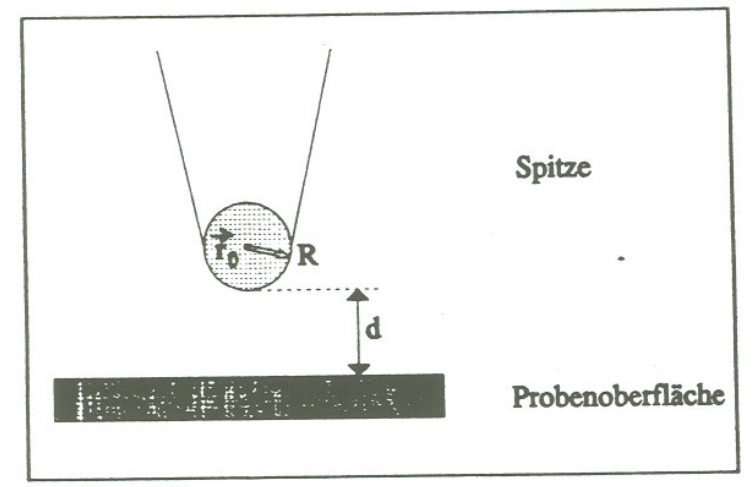
\includegraphics[width=14cm]{pics/tersoff_hamann}
    \caption{Das sogennante Tersoff-Hamann Standardmodell, welches in
        der Modellierung für die Rastertunnelmikroskopie in der Näherung
        für eine räumlich ausgedehnte Tunnelspitze herangezogen wird.
        Abbildung aus \cite{staatsexamen}.}
\label{fig:tersoff_hamann}
\end{figure}

\subsection{Charakterisierung von Kristallgittern}
Vor der Beschreibung der Oberflächen von Kristallen wenden wir uns dem darunter liegenden 
Gitter zu, das die Basis für die Oberfläche darstellt. Die charakteristischen Größen 
sind auch für die Oberflächen wichtig. Die Untersuchung der Kristallgitter findet vor 
allem durch Beugungsexperimente statt, da diese die periodische Struktur am besten 
ausnutzen und so zu höherer Genauigkeit kommen als direkte Abbildung der Oberflächen. 

Fundamental für die Beschreibung der Phänomene der Festkörperphysik ist der reziproke 
oder $\K$-Raum. Er ist aus den $\K$-Vektoren ebener Wellen aufgebaut, die mit 
$\ex{i \K \cdot \R}$ beschrieben werden. Sind nun 
die Gittervektoren eines Kristalles im Ortsraum mit $\A_1,\ \A_2,\ \A_3$ gekennzeichnet, 
so gilt für die reziproken Gittervektoren $\g_1,\ \g_2,\ \g_3$:
\begin{eqnarray}
    \g_1 = 2 \pi \frac{\A_2 \times \A_3 }
        {\A_1\cdot (\A_2 \times \A_3)} \qquad \mathrm{und \ zyklisch} \\
    \mathbf{g_i} \cdot \mathbf{a_j} = 2 \pi \delta_{ij}
\end{eqnarray}
Die periodische Struktur des Kristalles bleibt also im reziproken Raum erhalten.
Ein beliebiger Vektor $\G$ des reziproken Gitters lässt sich als ganzzahlige Linearkombination 
der Basisvektoren darstellen.
\begin{equation}
    \mathbf{G} = h \mathbf{g_1} + k \mathbf{g_2} + l \mathbf{g_3} \mbox{ mit }h,k,l \in \mathbb{Z}
\end{equation}
Für einen Vektor $\R$, der auf dem Gitter im Ortsraum liegt, gilt dann also:
\begin{eqnarray}
    \mathbf{r} &=& n_1 \mathbf{a_1} + n_2 \mathbf{a_2} + n_3 \mathbf{a_3} \\
    \mathbf{G} \cdot \mathbf{r}&=& 2 \pi m  \\
    n_1, \, n_2, \, n_3, \, m &\in& \mathbb{Z}
\end{eqnarray}

Schließlich lässt sich jede Funktion, die im Ortsraum periodisch ist, als 
Fourierreihe im reziproken Raum darstellen:
\begin{equation}
    f(\R) = \sum_{\G} F_{\G} \ex{i \G \cdot \R}
\end{equation}

Bei der Bezeichnung der Netzebenen werden die sogenannten Millerschen Indizes benutzt. 
Spannt man mit drei nicht auf einer Geraden liegenden Gitterpunkten eine Ebene, so ist 
diese durch 
drei ganze Zahlen $m, n, o$ gekennzeichnet. Aus diesen erhält man ein teilerfremdes 
Triplet $(h, k, l)$, indem man die reziproken Werte $h' = 1/m, k' = 1/n, l' = 1/o$ mit 
einer ganzen Zahl $p$ multipliziert. Der reziproke 
Gittervektor $\G$ steht nun senkrecht auf dem mit $(h, k, l)$ beschriebenen Gitter.
\cite{ibach2009festkorperphysik}


\subsection{Blochtheorie und Bändermodell}

Für die Rastertunnelmikroskopie ist die räumliche Verteilung der Elektronen an 
der Oberfläche von zentraler Bedeutung. Die Blochtheorie macht Aussagen über 
die Aufenthaltswahrscheinlichkeiten von Elektronen in periodischen 
Gittern und liefert ein Modell zur Erklärung des Bändermodells. 
Für ein Elektron mit Wellenfunktion $\psi$ gilt bei Vernachlässigung der 
Elektron-Elektron-Wechselwirkung in der nichtrelativistischen Näherung die 
Schrödingergleichung 
\begin{equation}
    \hat H \psi(\R) = \Big[ - \frac{\hbar^2}{2m} \Delta + V(\R) \Big] \psi(\R) = E \psi(\R)
\end{equation}
mit periodischem Potential
\begin{equation}
    V(\R) = V(\mathbf{r + r_n}); 
\qquad \mathbf{r_n} = n_1 \mathbf{a_1} + n_2 \mathbf{a_2} + n_3 \mathbf{a_3} 
\end{equation}
wobei $\mathbf{a_i}$ Gittervektoren des Ortsraumes sind. Auf Grund der Periodizität lässt 
sich das Potential in eine Fourierreihe zerlegen:
\begin{eqnarray}
    V(\R) &= &\sum_\G \VG \mathrm{e}^{i\G \cdot \R} \\
    \mathrm{mit \ Fourierkomponente \quad}  \VG &= &\frac{1}{L} \int \mathrm{e}^{i\G \cdot \R} 
    V(\R) \mathrm{d}\R  \nonumber \\
    \mathrm{und \ reziprokem \ Gittervektor \quad} \G &= &h\mathbf{g_1} + k\mathbf{g_2} +l\mathbf{g_3}; 
    \quad h, \ l, \ k, \ \in \mathbb{Z}. \nonumber
\end{eqnarray}

Der Ansatz für die Lösung ist eine Linearkombination ebener Wellen
$ \psi(\R) = \sum_\K C_\K \mathrm{e}^{i\K \cdot \R}, $
für die nach Einsetzen in die Schrödingergleichung gelten muss:
\begin{equation}
    \sum_\K \mathrm{e}^{i\K \cdot \R} 
    \Big[ \Big( \frac{\hbar^2 k^2}{2m} - E\Big) C_\K + \sum_\G \VG C_{\K - \G}\Big] 
    = 0
\end{equation}
Aus der Unabhängigkeit von $\R$ folgt dann
\begin{equation}
    \Big( \frac{\hbar^2 k^2}{2m} - E\Big) C_\K + \sum_\G \VG C_{\K - \G}= 0
\end{equation}

Zu jeden $\K$ Wert ergeben sich also $N$ Gleichungen, die die Koeffizienten
$C_\K$ jeweils mit $C_{\K - \G'}$, $C_{\K - \G''}$,\ldots  koppeln, wobei $N$ die Anzahl 
der Elementarzellen im Gitter ist. Daher lassen sich die Wellenfunktionen 
mit Energie $E_\K$ also Superposition ebener Wellen schreiben, deren $\K$ Werte 
alle auf dem reziproken Gitter liegen: 

\begin{eqnarray}
    \psi_\K(\R)&=& \sum_\G C_{\K - \G} \mathrm{e}^{i(\K - \G) \cdot \R} \nonumber \\
            &=& \sum_\G C_{\K - \G} \mathrm{e}^{i \G \cdot \R}  \mathrm{e}^{i\K \cdot \R} \nonumber \\
            &=& u_\K(\R) \cdot \mathrm{e}^{-i\K \cdot \R} 
\end{eqnarray}

Diese Wellenfunktionen werden Bloch-Wellen genannt. Das Bloch-Theorem sagt aus, 
dass für das Einelektronenproblem im periodischen Potential eben diese Bloch-Wellen 
Energie-Eigenfunktionen mit Eigenwerten $E_\K$ mit $\K = \frac{2 \pi}{L} (n_x, n_y, n_z)$ und
\begin{equation}
    u_\K(\R) = u_\K(\mathbf{r + r_n}) 
\end{equation}
sind. Es folgt direkt 
\begin{equation}
    \psi_{\K + \G}(\R) = \psi_\K(\R) 
\end{equation}
und damit auch: 
\begin{equation}
    E(\K) = E(\K + \G)
\end{equation}
Für die Aufenthaltswahrscheinlichkeit folgt $|\psi(\mathbf{r})|^2 = |u|^2$ - wir können also 
die Elektronendichte als Messgröße für die Positionen der Atomrümpfe verwenden!

Mit Hilfe der Näherung für ein quasifreies Elektron liefert die Bloch-Theorie auch einen 
Ansatz für die Erklärung der Bänderstruktur in Festkörpern. Dafür gehen wir von einem freien 
Elektron aus, für das jedoch weiter die Periodizität im Raum gelten soll (das sog. \emph{'leere Gitter'}). 
Verschieben wir nun unser Gitter um einen reziproken Gittervektor $\G$, so ließt sich die 
Schrödingergleichung im $\K$-Raum wie folgt:
\begin{eqnarray}
    \Big(E - \frac{\hbar^2}{2m}|\K - \G|^2\Big) C_{\K - \G} &=&
        \sum_{\G'} V_\mathbf{G' - G} C_{\K - \G'}, \quad \mathrm{d.\ h.} \nonumber \\
    \label{eqn:bloch1}    
    C_{\K - \G} &=& \frac{ \sum_{\G'} V_\mathbf{G' - G}}{E - \frac{\hbar^2}{2m}|\K - \G|^2} 
\end{eqnarray}


Gehen wir nun von einer Störung des Falles eines freien Elektrons aus, so können wir 
die eigentliche Energie in erster Näherung durch $E = (\hbar^2 k^2) / (2m)$ ersetzen. 
Da wir nur die größten Koeffizienten $C$ betrachten, sollte der Nenner 
in \eqref{eqn:bloch1} möglichst klein werden, es sollte also die Beziehung 
\begin{equation}
    E(\K) = E(\K + \G)
\end{equation}
gelten, die genau die Braggbedingung für Reflexion ist. D.~h. die stärkste Abweichung zum freien 
Elektron treten dann auf, wenn der $\K$ Vektor auf dem Rand der sog. \emph{1. Brillouin-Zone} liegt. 
Weiterhin folgt mit $V_0 = 0$ durch einsetzen von $\G = 0$ in \eqref{eqn:bloch1}, dass auch $C_\K$ in der ersten Ordnung 
beträgt. Daher ergibt sich das Gleichungssystem 
\begin{eqnarray}
    \psi_\K(\R)&=& \sum_\G C_{\K - \G} \mathrm{e}^{i(\K - \G) \cdot \R} \nonumber \\
            &=& \sum_\G C_{\K - \G} \mathrm{e}^{i \G \cdot \R}  \mathrm{e}^{i\K \cdot \R} \nonumber \\
            &=& u_\K(\R) \cdot \mathrm{e}^{-i\K \cdot \R} 
\end{eqnarray}

welches die Determinantengleichung 
\begin{eqnarray}
    \begin{vmatrix}
        \Big(\frac{\hbar^2}{2m} k^2 - E\Big) & \VG \\
        V_\mathbf{-G}   & \Big(\frac{\hbar^2}{2m} |\K - \G|^2 - E\Big) 
    \end{vmatrix} = 0; \\
    E_{\K - \G}^0 = \frac{\hbar^2}{2m} |\K - \G|^2 \nonumber
\end{eqnarray}
mit den Lösungen 
\begin{equation}
    E^\pm = 
    \frac{1}{2}(E_{\K - \G}^0 + E_\K^0) \pm 
        \frac{1}{2}\Big[(E_{\K - \G}^0 + E_\K^0)^2 + |\VG|^2\Big]^{\frac{1}{2}}
\end{equation}

auflöst. Unmittelbar auf dem Rand der 1. Brillouin-Zone gilt $E_{\K - \G}^0 = E_\K^0$ und 
damit für die Energiedifferenz der Bänder: 
\begin{equation}
    \Delta E = E^+ - E^- = 2 |\VG|
\end{equation}
Für den eindimensionalen Fall ist das in Abb.~\ref{fig:bloch} schematisch dargestellt.
\cite{ibach2009festkorperphysik} 

\begin{figure}[!t]
  \begin{captionbeside}[]{Darstellung der Aufspaltung der Energieparabel des freien Elektrons 
(gestrichelt) an den Rändern der 1. Brillouin-Zone im Rahmen der störungestheoretischen 
Betrachtung von Elektronen in periodischen Gittern (hier für den eindimensionalen Fall). 
(1) und (2) markieren die jeweiligen Bänder. 
Aus \cite{ibach2009festkorperphysik}.}[r]
    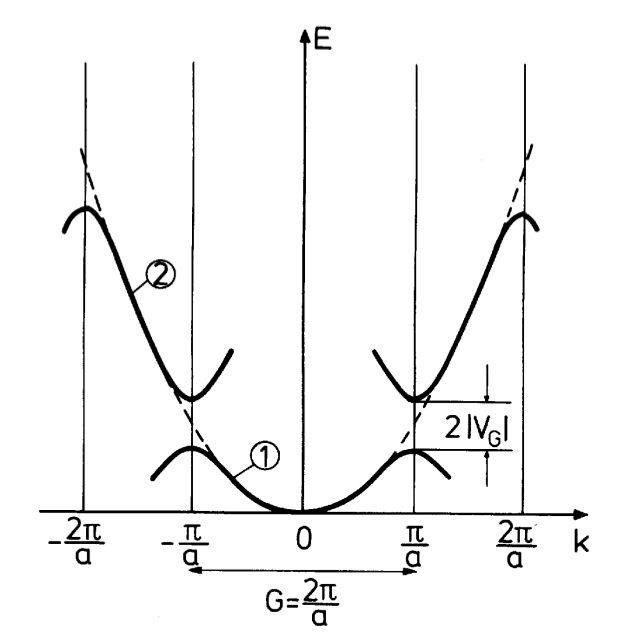
\includegraphics[width=0.5\textwidth]{pics/bloch}
  \end{captionbeside}
  \label{fig:bloch}
\end{figure}

Im Kristall gibt es nun Abweichungen von dem Modell. Zuerst einmal haben Kristalle 
endliche Ausdehnungen, sodass das zuvor als kontinuierlich angenommene 
Energiespektrum diskret ist. Zweitens haben die Elektronen eine Wechselwirkung. 
Diese ist gering im Vergleich zum Potenzial der Kerne, allerdings sorgt sie dafür, 
dass sich die erlaubten Energiewerte für Elektronen eines einzelnen Atoms aufspalten 
in $N$ sehr nahe beieinander liegenden Werten. Für große $N$ sind die erlaubten 
Energiewerte in dem so entstandenen \emph{Band} nahezu kontinuierlich, 
siehe Abb.~\ref{fig:baender1}. Pro Band können  
sich nach dem Pauliprinzip und unter Berücksichtigung des Spins maximal 2N Elektronen 
befinden. Geht die Temperatur gegen Null, so sind die Elektronen in der Konfiguration 
mit der niedrigsten möglichen Gesamtenergie angeordnet. Das oberste dann voll mit 
Elektronen besetzte Band wird als \emph{Valenzband} bezeichnet. Wird die Temperatur 
erhöht, so steht thermische Energie zu Verfügung. Die maximal Energie, die Elektronen 
im Mittel erhalten würden, wenn erlaubte Energiezustände vorhanden wären, wird als 
\emph{Fermienergie} bezeichnet. 
Liegt das Energieband über dem Valenzband unterhalb der Fermienergie oder hat sogar 
einen Überlapp mit dem Valenzband, so können Elektronen Enrgie aufnehmen und in dieses 
Band gelangen. Dort sind sie räumlich deutlich schwächer gebunden und können bei einem 
von außen angelegtem Feld in Richtung des Feldes driften. Daher wird das Band über dem 
Valenzband als \emph{Leitungsband} bezeichnet. Metalle sind deshalb elektrische Leiter, weil 
bei ihnen Leitungs- und Valenzband überlappen. Für das einwertige Natrium ist beispielsweise 
das oberste besetzte Band, das sich aus den 3$s$-Orbitalen zusammensetzt, nur halb besetzt. 
Für zweiwertige Metalle wie Magnesium überlappen sich Leitungs- und Valenzband. 
Bei Isolatoren liegt die Fermienergie niedriger als die untere Kante des Leitungsbandes. 
Die Elektronen können keine Energie eines angelegten Feldes aufnehmen und es kann kein 
Strom fließen. Bei Halbleitern ist die Fermienergie ab einer bestimmten Energie höher 
als die niedrigste Energie des Leitungsbandes. Daher ist ihre Leitfähigkeit 
temperaturabhängig. Siehe Abb.~\ref{fig:baender2}.\cite{demtroder2000experimentalphysik}\\ 

\newcommand{\picwidththeo}{0.48\textwidth}

\begin{figure}
    \centering
    \begin{subfigure}[b]{\picwidththeo}
        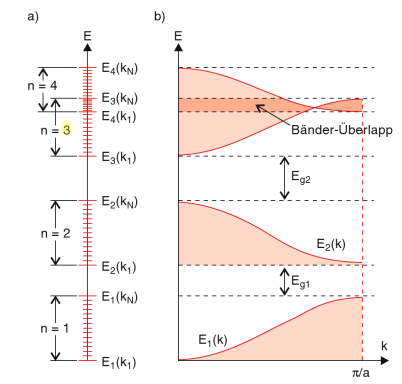
\includegraphics[width=\textwidth]{pics/baender1}
        \caption{Zur Entstehung der Energiebänder. Dargestellt ist die Aufspaltung der erlaubten 
Energiewerte von $N$ Elektronen im Kristall. 
(a) Eindimensionale Darstellung, 
(b) Darstellung von $E_n(k)$, die gestrichelte Linie ist die Grenze der 1. Brillouin-Zone;
aus \cite{demtroder2000experimentalphysik}}
        \label{fig:baender1}
    \end{subfigure}\qquad
    \begin{subfigure}[b]{\picwidththeo}
        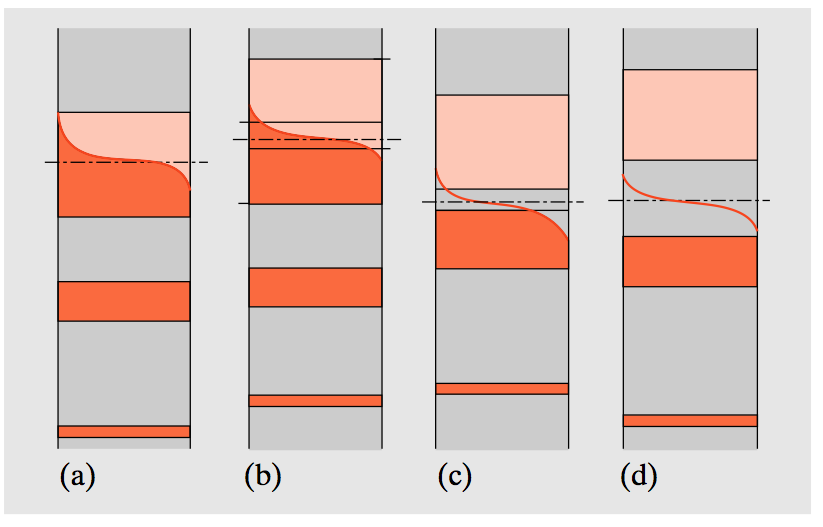
\includegraphics[width=\textwidth]{pics/baender2}
        \caption{Vereinfachte Darstellung des Bändermodells für 
(a) Metalle der ersten Hauptgruppe (Alkalimetalle), 
(b) Metalle der zweitern Hauptgruppe (Erdalkalimetalle), 
(c) Halbleiter (im leitfähigen Zustand)
(d) Isolatoren
aus \cite{vogel1997gerthsen}}
        \label{fig:baender2}
    \end{subfigure}
    \caption{Schemata zum Bändermodell}\label{fig:baender}
\end{figure}



\subsection{Grundlagen der Festkörperoberflächen}
Das zuvor angenommen, unendlich ausgedehnte, periodische Kristallgitter spielt 
bei der Untersuchung der Oberflächen nur noch eine untergeordnete Rolle – 
schließlich ist eine Oberfläche zunächst einmal eine Abweichung dieser 
Eigenschaft. Im Allgemeinen kann es Abweichungen in null, ein, zwei oder drei 
Dimensionen geben. Letztere sind Abweichungen der unterliegenden Baustruktur, 
die zum Teil eine Mosaikstruktur bilden, die sich auch auf größere Skalen 
erstrecken. Zweidimensionale Strukturen tauchen als großflächige 
Überstrukturen oder kleinere Facetten auf. Eine Kategorisierung verschiedener 
Oberflächen wird von Henzler und Göpel \cite{henzler1991oberflachenphysik} 
gegeben (Abb.:~\ref{fig:oberflaeche}).
In jedem Fall erfahren die Atome der Oberfläche nicht mehr das 
regelmäßige Potential von allen Seiten. Dies resultiert je 
nach Art als Oberflächenrelaxation oder -rekonstruktion. 
Ersteres bezeichnet lediglich eine globale Verschiebung der oberen Schicht 
gegen die Basis, beispielsweise normal oder lateral, wobei die Symmetrien 
der Oberfläche nicht verändert werden und sich die freie Energie verringert. 
Dieser Effekt wird bei den meisten Metallen beobachtet \cite{oura2003surface}. 
Abb. \ref{fig:Ag(110)} zeigt beispielsweise die relaxierte Oberfläche von Silber 
auf der (110)-Fläche.
Bei der Oberflächenrekonstruktion bilden sich meist größere Einheitszellen als die 
des darunter liegenden Kristalls. Bei Halbleitern hängt das oft damit zusammen, 
dass die Anzahl nicht abgesättigter Bindungen minimiert wird, so beispielsweise 
bei Silizium entlang der (100)-Fläche, bei der nach gedanklichem Aufspalten zwei 
Bindungen frei wären. Je zwei Atome verbinden sich zu sog. Dimeren, wobei die 
Oberfläche räumlich verzogen wird und sich volle bzw. leere Reihen mit einer 
Höhe von bis zu fünf Schichten und über große Entfernungen bilden 
\cite{chadi1979atomic}. Die bereits in der historischen Einleitung gezeigte 
Si-Oberfläche entlang der 
(111)-Ebene zeigt ebensfalls eine Oberflächenrekonstruktion, allerdings mit 
deutlich anderen Mustern. Die kubisch-flächenzentrierten Edelmetalle der 
6.~Periode, Ir, Pt und Au bilden als Ausnahme unter den Metallen ebenfalls 
Oberflächenrekonstruktionen, die sog. \emph{missing row}-Konstruktion, 
wie weiter unten bei der Beschreibung von Gold verdeutlicht wird 
\cite{kittel2013einfuhrung}. 

\begin{figure}[!t]
  \begin{captionbeside}[]{Rastertunnelkikroskop-Aufnahme mit atomare Auflösung einer reinen 
Silberoberfläche entlang der (110)-Fläche. Zu erkennen ist, dass die Oberfläche 
lediglich relaxiert ist, und Rekonstruktion stattfindet. 
Aus \cite{kahn:stm_images}.}[r]
    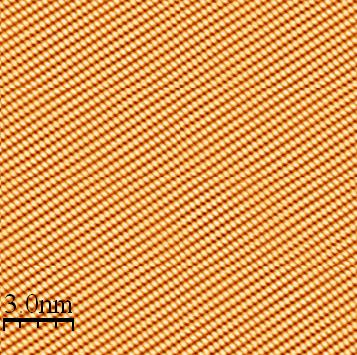
\includegraphics[width=0.5\textwidth]{pics/Ag(110)_clean}
  \end{captionbeside}
  \label{fig:Ag(110)}
\end{figure}

Zur mathematischen Beschreibung regelmäßiger Überflächen werden die Gittervektoren 
aus dem Ortsraum benutzt, die in der Oberfläche liegen. Ausreichend sind meistens 
jene aus der obersten Atomschicht. Die Atome befinden sich dann an den Positionen 
\begin{equation}
    \mathbf{r} = m_1 \mathbf{a_1} + m_2 \mathbf{a_2},
\end{equation}
wobei nach Konvention $|\mathbf{a_1}| \le |\mathbf{a_2}|$ und 
$\gamma = \angle (\mathbf{a_1}, \mathbf{a_2}) > 90 \deg$ der Winkel zwischen den 
beiden Vektoren ist. Da die Atome in einer Ebene liegen, ist die Anzahl möglicher 
Anordnungen, die sog. Bravais-Netze, deutlich kleiner als für einen 3D-Kristall. 
Es gibt genau fünf, wie in Abb.~\ref{fig:Bravais} gezeigt 
\cite{henzler1991oberflachenphysik}.
Zur vollständigen Beschreibung fehlen dann allerdings noch die Angaben zur Lage 
der Oberflächenatome relativ zur darunter befindlichen Basis. 

Zur Beschreibung der Oberfläche wird zuerst die ideale Oberfläche angenommen, 
die sich aus dem darunter liegenden Kristallgitter ergäbe, und deren Vektoren mit
$|\mathbf{a_1}| \le |\mathbf{a_2}|$ bezeichnet werden. Die tatsächliche Struktur, 
soweit periodisch, kann dann als Verhältnisse $\frac{\mathbf{a_1}}{\mathbf{b_1}}$, 
$\frac{\mathbf{a_1}}{\mathbf{b_1}}$ und Winkel zwischen Basis und Oberfläche angegeben 
werden. Zusammen mit der Millerschen Schreibweise für die Kristallfläche der Basis 
ergibt sich so eine kompakte Schreibweise, z.~B. 
$\mathrm{Si}(111)(\sqrt{3} \times \sqrt{3}) \mathrm{R} 30 \deg$. 
Ist diese Schreibweise ungeeignet aufgrund fehlender Symmetrien, so kann eine 
Matrixschreibweise benutzt werden. Sind die Einträge ganze Zahlen, so liegen die 
Atome der Oberfläche direkt auf der Basis. Bei rationalen Zahlen gibt es auch 
zwischen den Basisatomen Oberflächenatome, während bei irrationalen Zahlen die 
Oberfläche quasi unabhänging von der Basis gesehen werden muss. Sie wird dann auch 
als inkommensurabel bezeichnet\cite{henzler1991oberflachenphysik}.

\begin{figure}
    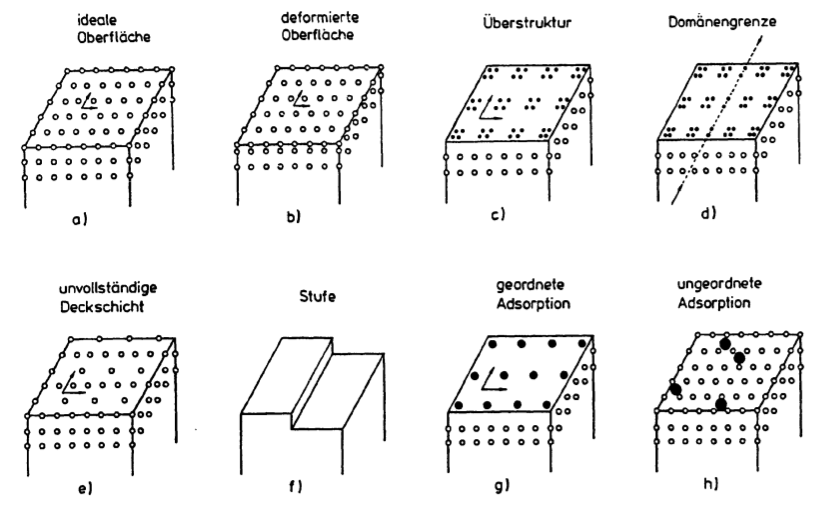
\includegraphics[width=1.0\textwidth]{pics/oberflaechenstruktur}
    \caption{Die ideale Oberfläche und einige mögliche Oberflächenstrukturen. 
Die ideale Oberfläche entspricht einer Gitterebene im Kristall, die defomierte 
Oberfläche entsteht durch Relaxation (hier in normaler Richtung) und wird bei den 
meisten Metallen beobachtet, während die Überstruktur ein Resultat der Rekonstruktion 
ist und z. B. bei Halbleitern oder Gold zu beobachten ist. 
Aus \cite{henzler1991oberflachenphysik} }
\label{fig:oberflaeche}
\end{figure} 
\begin{figure}
  \begin{captionbeside}{Bravais-Gitter zur Oberflächenstrukturbeschreibung. Die 
kleinstmöglichen Zellen sind in den unteren drei Gittern mit $\underline{a}_2^p$ 
beschriftet. 
Aus \cite{henzler1991oberflachenphysik}. }[r]
    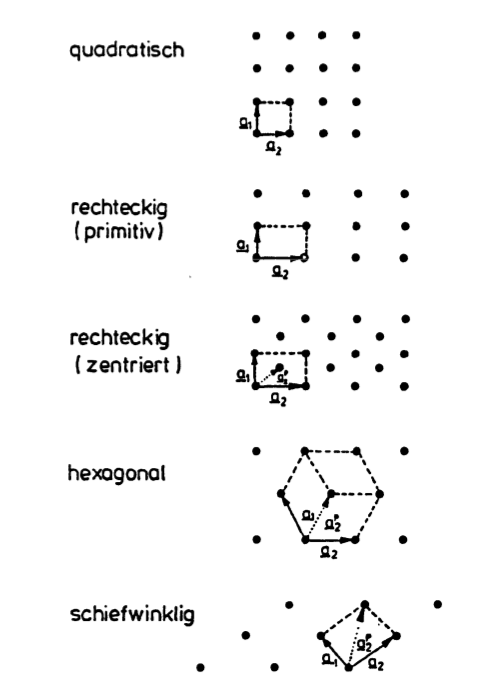
\includegraphics[width=0.5\textwidth]{pics/Bravais}
  \end{captionbeside}
  \label{fig:Bravais}
\end{figure} 


\subsection{Struktur von Graphit, Gold und $\mathrm{MoS_2}$}
Die Kristallstruktur von Graphit zeichnet sich vor allem durch seine Schichtenstruktur 
aus. Die Kohlenstoffatome sind in den aus kovalent gebundenen Sechsecken bestehenden 
Basalebenen oder Graphenschichten deutlich fester aneinander gebunden (4.3 eV), als 
an solche aus benachbarten Schichten (0.07 eV). Daher ist Graphit entlang dieser Linien 
sowohl mechnisch deutlich stabiler als auch sehr viel leitfähiger (für Wärme und 
elektrischen Strom). Die Unterschiede in der Bindungsenergie spiegeln sich auch in den 
Abständen wider: So sind nächsten Nachbarn innerhalb einer Schicht nur $0.142\mathrm{nm}$ 
entfernt, während die Schichten $0.335\mathrm{nm}$ auseinander liegen.  
Graphit tritt nicht nur in zueinander korrlierten Schichten auf, 
sondern auch unkorrliert (sog. turbostratischer Kohlenstoff). Die hier untersuchte Form 
ist jedoch regelmäßig - die Winkelabweichung für das verwendete HOPG (highly orientated 
pyrolytic graphite) beträgt weniger als $1 \deg$ \cite{mcnaught2000iupac}. Diese 
synthetische Form des Graphit wird auf Grund von ihrer Regelmäßigkeit und Reinheit 
heute zur Kalibrierung von Rastertunnelmirkoskopen verwendet \cite{lapshin1998automatic}. 
Es liegen in der Schichtung jedoch nicht alle Atome übereinander, sondern lediglich 
jedes zweite aus jedem Sechseck (siehe Abb.~\ref{fig:graphite}). 
Dadurch kommt es an der Oberfläche zu einem oft beobachteten 
Effekt: Anstatt sämtliche Atome der Sechsecke zu beobachten, taucht nur die Hälfte auf 
den STM-Bildern auf. Erklärt wird das dadurch, dass die Elektronendichte in der 
Fermienergie für Atome mit Nachbarn darunter höher liegt als bei solchen ohne
\cite{zeinalipour2008new}. Selloni~et~al.~\cite{Sellino1985} berechneten den Abstand 
der Atome mit bzw. ohne direkten Nachbarn in der Schicht darunter mit $0.15 \AA$. 

\begin{figure}
    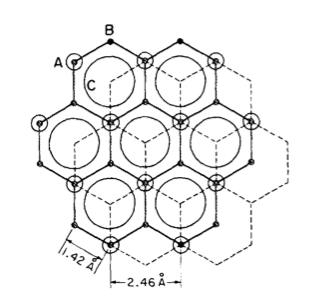
\includegraphics[width=0.7\textwidth]{pics/graphite}
    \caption{Hexagonale Oberflächenstruktur von Graphit. An den umkreisten Orten (A) 
liegen jeweils Atome aus der ersten und der zweiten Schicht übereinander, bei den 
übrigen (B) nicht. Bei STM-Aufnahmen sind fast ausschließlich die Atome mit Nachbarn 
zu erkennen, da hier Elektronen nahe der Fermienergie räumlich weiter oben liegen. 
Aus \cite{park1986tunneling}}
    \label{fig:graphite}
\end{figure} 

Gold ist als kubisch-flächenzentriertes Kristallgitter aufgebaut. Die Gitterkonstante 
beträgt $407.82\mathrm{pm}$\cite{ohring1995engineering}. Im Gegensatz zum Graphit 
treten jedoch beim Gold enorme Veränderungen der Oberflächenstruktur gegenüber der 
darunter liegenden Basis auf. Auf einer (110)-Fläche wurde die Bildung von 
(111)-Facetten beobachtetet, die Kanälevon meistens zwei bis vier Schichten Tiefe 
formen. Gleichzeitig ist die Oberfläche von Stufen gekennzeichnet, die sowohl parallel 
als auch normal zu den Kanälen verlaufen, siehe Abb. \ref{fig:Au(110)_channels}. Die Darstellung 
der Oberfläche mit dem Rastertunnelmikroskop ist auf Grund der metallischen Struktur 
deutlich schwieriger als bei Halbleitern, da die Elektronen aus dem Leitungsband kaum 
räumlich lokalisiert sind. 

\begin{figure}
    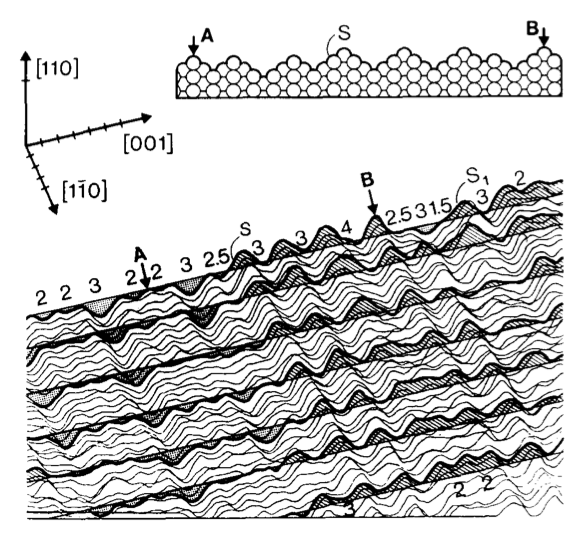
\includegraphics[width=0.6\textwidth]{pics/Au(110)_channels}
    \caption{Rastertunnelmikroskop-Aufnahmen von Gold(110)-Oberfläche mit 
Rekonstruktion. Die Geraden verdeutlichen die abschüssige Terassenstruktur, die 
Nummern die Tiefe der Kanäle (in Vielfachen der Ebenenabstände). Bei $\mathrm{S}$
und $\mathrm{S_1}$ befinden sich Stufen mit Höhe einer Atomlage. An den Kristallaxen 
ist der Maßstab gekennzeichnet: ein Schritt entsprechen 5 \AA. Über der Aufnahme 
deutet ein schematischer Querschnitt die Struktur der Kanäle an. 
Aus \cite{binnig1983111}.}
    \label{fig:Ag(100)}
\end{figure} 

Molybdänit ($\mathrm{MoS_2}$, auch Molybdän(IV)-sulfid) ist ein Halbleiter mit 
hexagonalem Kristallgitter der Raumgruppe $\mathrm{P \, 6_3/mmc}$. Ähnlich 
dem Graphit gibt es eine schichtartige Struktur, auch hier können die Schichten 
relativ leicht gegeneinander verschoben werden. Die Gitterparameter sind mit 
$a = 3.161 \AA$ sowie $c = 12.295 \AA$ angegeben, siehe
Abb.~\ref{fig:MoS2_structure} \cite{schrocke1981mineralogie}. 
Auf Gund der Schichtstruktur findet $\mathrm{MoS_2}$ als 
Schmiermittel Verwendung und kann wie Graphen als einatomige Schicht isoliert 
werden, sodass es mögliches Transitormaterial gehandelt wird 
\cite{mak2010atomically}. 

\begin{figure}
  \begin{captionbeside}{Gitterstruktur von $\mathrm{MoS_2}$, Ausschnitte aus drei übereinander 
liegenden Schichten mitsamt Koordinationspolyedern. Für die Abstände gilt 
$a_1 = a_2 = a_3 = 3.161\AA =: a$ und $c_0 = 12.295\AA$. 
Aus \cite{schrocke1981mineralogie}.}[r]
    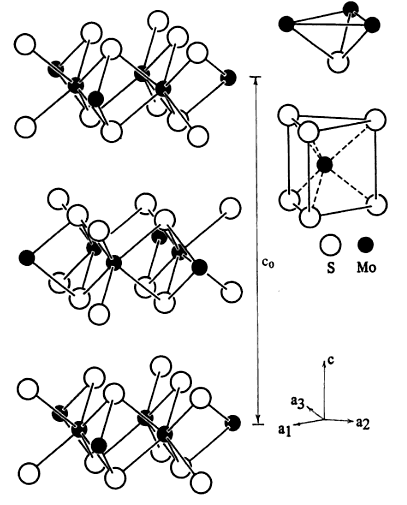
\includegraphics[width=0.5\textwidth]{pics/MoS2_structure}
  \end{captionbeside}
  \label{fig:MoS2_structure}
\end{figure} 

\section{Aufbau des Versuchs}
\begin{figure}[h]
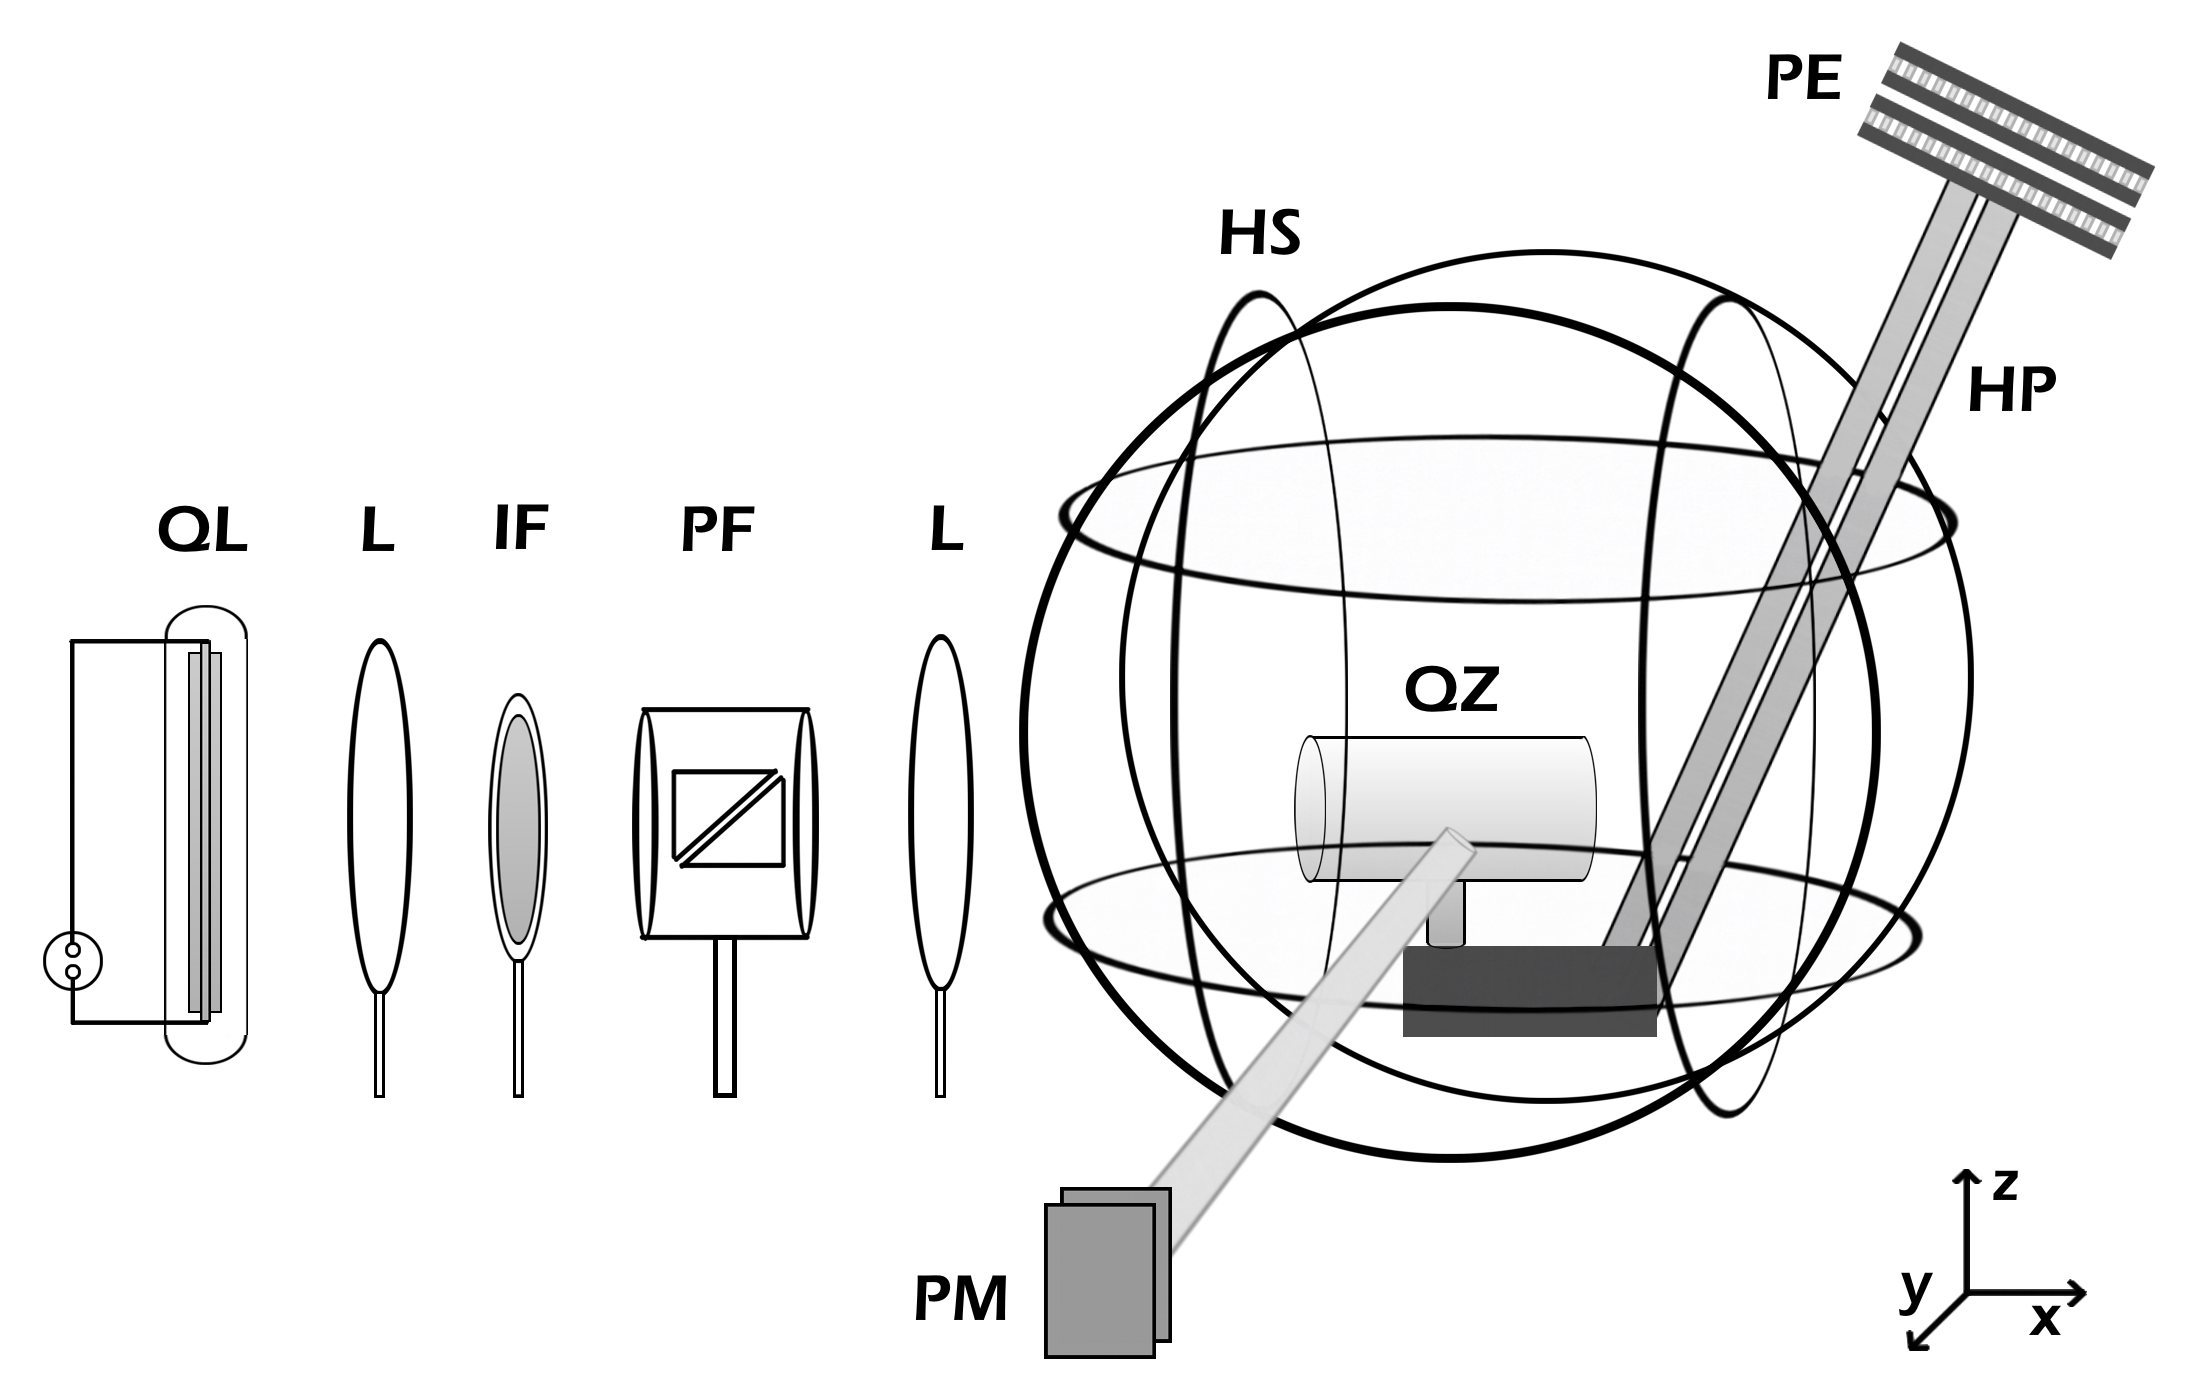
\includegraphics[scale=0.3]{Bilder/aufbau}
\caption{Aufbau. Quelle: [ver]}
\end{figure}
Im Versuch soll die Lebensdauer des durch Licht der Wellenlänge $253,7nm$ angeregten $^{3}P_{1}$-Zustandes von Quecksilber untersucht werden. Dazu benutzt man eine Quecksilberdampf- Niedrigdrucklampe (QL). Das so erzeugte Licht wird von der ersten Linse (L) kollimiert und von der zweiten fokussiert. Zwischen diesen Linsen ist ein Interferenzfilter (IF) angebracht, welche einen Durchlassbereich von $(255\pm5)nm$ FWHM  verwendet und somit die gewünschte Wellenlänge durchlässt. Besonders wichtig ist dabei, dass eine Wellenlänge von $184,5 nm$ herausgefiltert wird, da diese den sonst dominierenden Übergang von Quecksilber zwischen $^{1}P_{1}$ und $^{1}S_{0}$ anregen würde. Ein doppelbrechender Polarisationsfilter (PF) ermöglicht die Wahl der Polarisationsrichtung.\\
Das Licht trifft auf eine Quecksilberdampf-Resonanzzelle (QZ), welche aus einem Quarzkolben und einer Vertiefung im Boden besteht, in welcher sich das Quecksilber sammelt. Zur Kühlung der Zelle werden Peltierlemente (PE) verwendet. Aufgrund ihres elektrischen Störfeldes werden diese mithilfe wärmetransportierender 'Heat Pipes' (HP) möglichst weig weg von der Zelle positioniert. Ebenfalls außerhalb ist ein Photomultiplier (PM) angebracht, welcher über den Photoeffekt das Fluoreszenzlicht in ein elektrisches Signal umwandelt und durch einen Potentialgradienten und mehreren Elektroden das Signal verstärkt.\\
Zur Kompensation von Hintergrund-Magnetfeldern werden zwei Paare von Helmholtz-Spulen (HS) benutzt und ein drittes dient zum Durchfahren des magnetisches Feldes, welches für das Hanle-Signal sorgt.

\section{Durchführung des Versuchs}
In Abbildung~\ref{fig:stm1} sehen wir das RTM, welches in der
folgenden Versuchsdurchführung verwendet wurde. Es handelt sich
um das Modell \textit{easyScan 2 STM, Version 1.6} welches von 
der Firma \textit{Nanoscience Instruments, Ink.} vertrieben wird.
Laut der Beschreibung des Herstellers 
bilden hunderte \textit{easyScan 2 STMs} einen
\textit{unersetzlichen} Bestandteil in der Lehre von Physik,
Chemie und Materialwissenschaften, werden aber auch in der
Forschung und Entwicklung eingesetzt. Anwendung findet das RTM
in der Spektroskopie sowie in der Grundlagenforschung.
In unserem Versuch spielt das easyScan 2 STM insofern eine Rolle,
dass es ohne weitere Zwischeninstanzen direkt die gemessen
Abstände in ein Bild auf dem Computer sendet. Diese Bilder
enthalten schon alle für den Versuch notwendigen Informationen,
die Parameter können auch direkt von dem bereitgestellten Programm
konfiguriert werden. Der Wandel vom ersten RTM, in dem die Dämpfung
noch von Supraleitenden Magneten und einer Vakuumkammer hergestellt
werden musste, zum diesem Modell und diese Fortschritt kommt uns
in unserem FP zu Gute. Die Spezifikationen des Modells 
(Ausschnitt, entnommen aus dem beiliegendem Handbuch):\\
\begin{table}[h]
\begin{tabular}{| l | p{7cm} |}
\hline
  Größe des Controllers, Gewicht: & 470x120x80 mm / 2.4 Kg\\ \hline
  Leistung & 90- 240 V~/ 30 W 50/60 Hz \\ \hline
  Rastergeschwindigkeit & Bis zu 60ms pro Linie mit 128 Datenpunkten  pro Linie \\ \hline
Rasterfläche & bis zu 2048x2048 Punkten \\ \hline 
Darstellungsmöglichkeiten: & Liniengraph, Farbplot und 3D Perspektive \\ \hline
Abbildungsmodi & Konstante Stromstärke (\textit{Constant Current}),
konstante Höhe (\textit{Constant Height}) \\ \hline
Maximale Auflösung in Z/ XY & 3pm/ 7.6pm \\ \hline
Maximaler Rasterumfang in Z/ XY & 200nm/ 500nm  \\ \hline
Maximale Probengröße & 10mm Durchmesser \\ \hline
Spitzenspannung & max. $\pm 10V$ in 5mV Schritten \\ \hline
\end{tabular}
\caption{Spezifikationen des Modells \textit{easyScan 2 STM}}
\label{tab:STM}
\end{table}

\begin{figure}
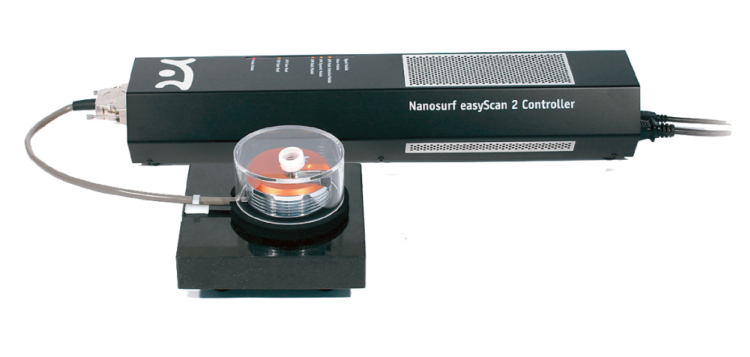
\includegraphics[width=14cm]{pics/stm1}
\caption{Photographie des verwendeten RTMs \textit{easyScan 2
STM Version 1.6} (entnommen aus Webseite des Herstellers)} 
 \label{fig:stm1}
\end{figure}

Da die Messaparatur für unseren Versuch schon aufgebaut worden
war und nicht modifiziert werden sollte, werden wir hier nicht
auf die einzelnen Komponenten des \textit{easy Scan 2 STM} Systems
eingehen, sondern nur die für unseren Versuch relevanten 
Bauteile beschreiben.
\subsection{Versuchsaufbau}
In Abbildung~\ref{fig:Rasterkopf} ist der Rasterkopf ds RTMs zu
sehen. Über den Probenhalter mit dazugehörigem Fixierungsmagneten
wird die Probe selbst angebracht; an den Spitzenhalter mit
Klammer die Spitze aus Platin-Iridiumdraht, 
welche wir für die Messungen selbst herstellt haben (siehe
Abbildung~\ref{fig:prepare_tip} und Abbildung~\ref{SEM_tip_picture}).
Der Probehalter stellt einen Zylinder dar, an dessen Kopf mithilfe
eines Magneten die Probe, welche im Idealfall auf einer dafür
passenden, ebenfalls magnetischen Schablone angebracht ist, 
befestigt wird, nachdem die Spitze angebracht wurde. 
Das Anbringen der Spitze erfolgt mit dafür passenden Zangen,
indem die Klammer angehoben, die Spitze eingelegt und mit
der Klammer fixiert wird.

\begin{figure}
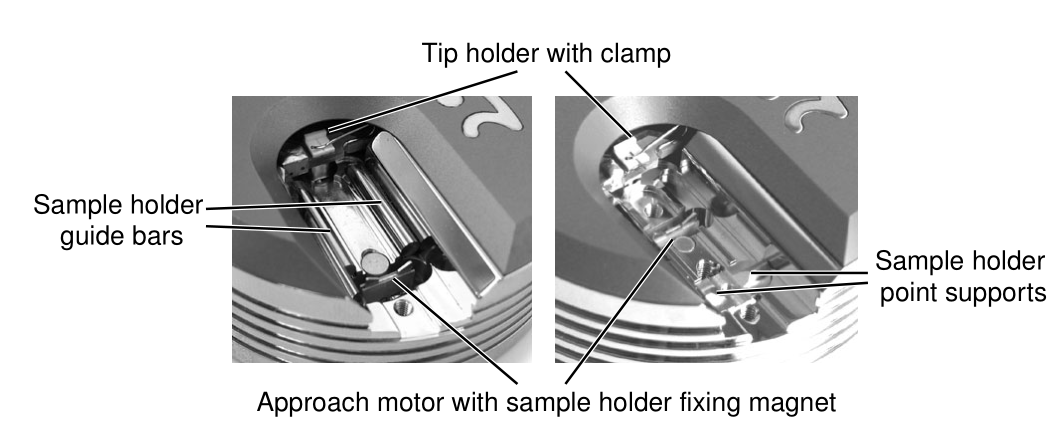
\includegraphics[width=14cm]{pics/rasterkopf}
\caption{Rasterkopf des RTMs \textit{easyScan 2
STM Version 1.6} (entnommen aus Webseite des Herstellers)
Zu sehen ist der Probenhalter (\textit{Sample holder}) mit dazu
gehörendem Annäherungsmotor (\textit{Approach motor} sowie
dem Fixierungsmagneten ({Fixing Magnet}), sowie dem Spitzenhalter
mit Klammer (\textit{Tip holder with clamp}). Die Funktionsweise
wird im Text beschrieben.}
 \label{fig:Rasterkopf}
\end{figure}

\begin{figure}
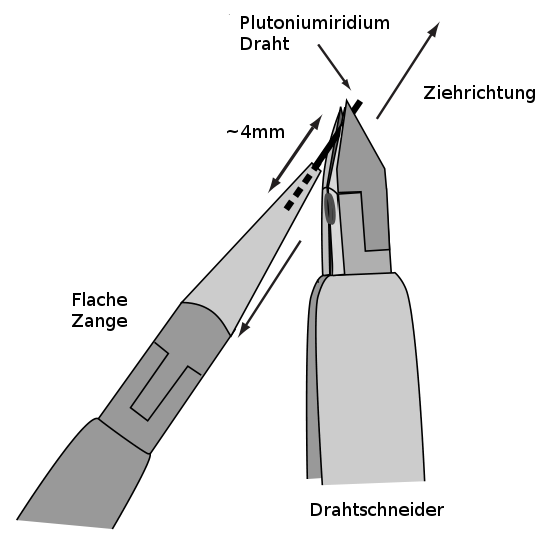
\includegraphics[width=10cm]{pics/prepare_tip2}
\caption{Vorbereitung des Drahtes. 1) Zunächst sollten die
zur Herstellung der Spitze notwendigen Werkzeuge mit Ethanol
gereinigt werden, von nun an sollte nur der Draht damit berührt 
werden. 2) Nun sollte der zu verknappende Draht mit den Zangen
gehalten werden, 3) dem Drahschneider umschlossen, aber nicht
abgezwickt, 4) in die angegebene Richtung \textbf{gezogen}, 5)
und endlich \textbf{abgerissen} werden, mit dem Ziel eine 
einatomige Spitze zu erzeugen (siehe Abbildung~\ref{fig:SEM_tip_picture})}
 \label{fig:prepare_tip}
\end{figure}

\begin{figure}
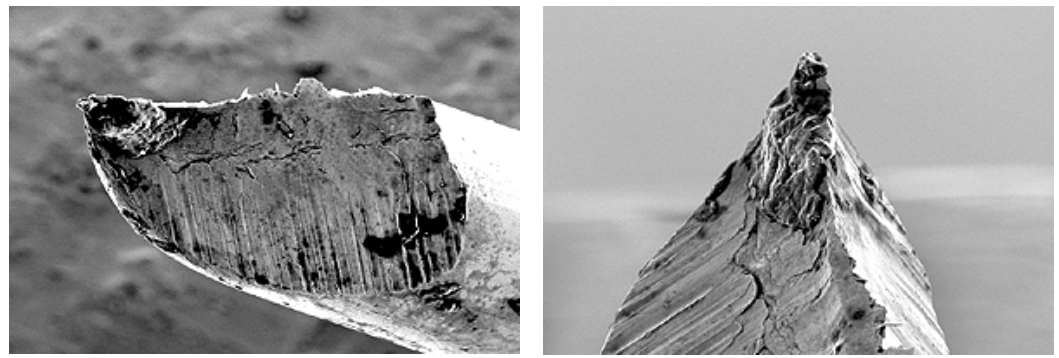
\includegraphics[width=10cm]{pics/SEM_tip_picture}
\caption{Das in Abbildung~\ref{fig:prepare_tip} beschriebene
Verfahren hat zum Ziel, eine möglichst präzise Spitze herzustellen.
Hier eine \textit{Scanning Electron Microskope} Abbildung
aus der Bedingungsanleitung des RTMs 
einer solchen hergestellen, idealen Spitze. Wie deutlich erkennbar
ist, verjüngt sich die Spitze nach oben und bietet so unter 
Umständen die Möglichkeit, eine einatomige Tunnelverbindung
mit der Probe einzugehen.}
 \label{fig:SEM_tip_picture}

\end{figure}
\subsection{Durchführung der Messungen}
Sobald die Spitze angebracht und die Probe eingeführt wurde, 
kann der Annäherungsprozess der Spitze zu der Probe beginnen. 
Zunächst kann manuell mit einer groben Steuerung die Spitze
(visuell) so nah wie möglich an die Probe herangebracht werden.
Dabei ist es von Vorteil, wenn diese schon zu Beginn recht nahe
aneinander liegen. Danach startet man den automatischen
Annäherungsprozess,
der die Spitze solange mit einer jeweils eingestellten
Geschwindigkeit der Probe annähert, bis ein erster Tunnelstrom
(in der Regel 1 nA)
zwischen der Probe und der Spitze fließen kann.  
Dieser Annäherungsversuch verfügt über verschiedene Modi:
\begin{itemize}
    \item \textbf{\textcolor{orange}{orange}}:
            Der Annäherungsversuch ist noch
            nicht abgeschlossen
    \item \textbf{\textcolor{red}{rot}}: 
            Der Annäherungsversuch ist in dem Sinne
            gescheitert, dass die Spitze mit der Probe kollidiert
            ist und womöglich Schaden erlitten hat. 
    \item \textbf{\textcolor{green}{grün}}: 
            Der Annäherungsversuch
            wurde ohne Fehlermeldungen
            abgeschlossen und ist vermutlich geglückt;
            der Tunnelstrom fließt wie vorgegeben.
\end{itemize}
Der erste Annäherung genügt in der Regel nicht, die Probe
mit der gewünschten Auflösung betrachten zu können. Deswegen muss
sukzessiv die Distanz 
durch weitere Annäherungen verkleinert werden,
unter jeweils niedrigerer
Tunnelspannung und veringerter Annäherungsgeschwindigkeit, 
ohne dass dabei die Spitze mit der Probe kollidiert.
Wenn nun die Annäherung erfolgt ist, kann die Abrasterung
der Probe beginnen. Die Qualität des Kontakts zwischen Probe
und Spitze kann nun anhand verschiedener Kriterien beurteilt werden,
darunter die der Spitze umgebende Höhenlinie (siehe
Abbildung~\ref{fig:topography}).
\begin{figure}
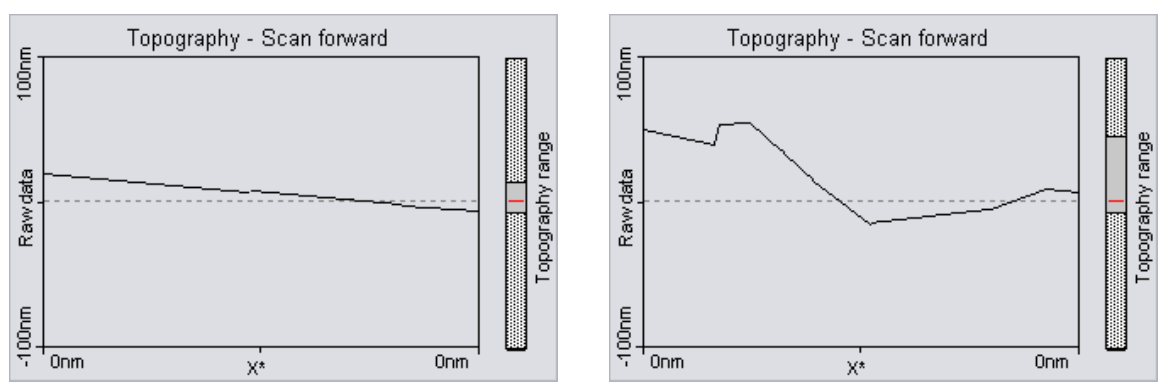
\includegraphics[width=14cm]{pics/Topography}
\caption{Screenshot aus dem Programm. Links zeigt eine 
Topographische Linie für einen guten Kontakt, während die
rechte ``nervöse'' Linie aufgrund ihrer Nichtlinearität
einen schlechten Tunneling Kontakt
andeutet, was auf eine zu stumpfe oder instabile Spitze
zurückgeführt werden kann.}
 \label{fig:topography}
\end{figure}
Wenn nun eine erfolgreiche Abrasterung mit zufriedenstellender
Auflösung vorliegt, kann ein Ausschnitt der Abrasterung
vergrößert werden, dieser Auschnitt wird dann erneut abgerastert
(sofern die technisch mögliche Auflösung nicht überschritten wird,
siehe Tabelle~\ref{tab:STM} auf Seite~\pageref{tab:STM}).



\clearpage
\section{Auswertung}
\subsection{Bestimmung der zeitlichen Verzögerungen}
Da hauptsächlich der NaJ-Szintillationszähler verwendet wird, wurden für diesen die zeitlichen Verzögerungen der Elektronik bestimmt. Diese wurden mithilfe der Diagramme, welche die jeweiligen Signale anzeigen, abgelesen (s. Anhang). \\
Die Verzögerung ist die zeitliche Differenz zwischen dem Einsatz der beiden Signale.\\
\subsubsection{Plastik-Szintillator}
Das Signal des Plastik-Szintillators wurde ohne Verstärkung bei einer Spannung von $U_{Plastik}=(1900\pm2)V$ vermessen. Das Signal hat eine periodische Form mit mehreren Peaks, wodurch die Verarbeitung und Auswertung des Signals erschwert wird. Dies ist auch der Grund, weshalb vornehmlich der NaJ-Szintillator verwendet wird.
\subsubsection{Verzögerung zwischen dem Amplifier-Eingang und dem unipolaren Ausgang}
Diese Verzögerung lasen wir zu $\Delta t=(3,7\pm0,5)\mu s$ ab. Der Fehler ergibt sich dabei durch die Ableseungenauigkeit.
\subsubsection{Verzögerung zwischen dem Amplifier-Eingang und dem bipolaren Ausgang}
Diese Verzögerung wurde zu $\Delta t=(1,5\pm0,5)\mu s$ bestimmt.
\subsubsection{Verzögerung zwischen dem Amplifier-Eingang und dem Ausgang des SCA}
Hierbei war eine Shaping Time von $3 \mu s$ eingestellt. Die Verzögerung wurde dann zu $\Delta t=(8,0\pm0,5)\mu s$ abgelesen. Bei Variierung der Shaping Time fiel auf, dass die Zeitdifferenz zwischen dem Ausgangssignal des Amplifier-Eingangs und dem Ausgang des SCA proportional zur Shaping Time ist. Dies bestätigt die Erwartung, da die Shaping Time eine Integrationsdauer angibt, über welche das Signal aufintegriert wird. \\
Bei den Ergebnissen handelt es sich natürlich nur um ungefähre Werte, deren Genauigkeit für eine qualitative Betrachtung allerdings ausreichend ist.
\clearpage
\subsection{Betrachtung des Untergrunds}
In den folgenden Schritten wurde jeweils der NaJ-Szintillationszähler verwendet. Da für diese eine Untergrundkorrektur benötigt wird, wurde für jeden Kanal des MCA die Zählrate $n_{u}=\frac{Counts~N}{Live~time~t}$ bestimmt. Dabei wurde statt der voreingestellten 'Real time' die 'Live time' verwendet, da diese die Dauer angibt, in welcher nicht gerade Pulse verarbeitet wurden und die Software somit unempfänglich für Counts war. Für die Untergrundmessung betrug die 'Live time' $t=32333 s$.\\
 Der Fehler der Counts berechnet sich, wenn man den Fehler auf die Zeit vernachlässigt, mithilfe der Gauss'schen Fehlerfortpflanzung zu $s_{n_{u}}=\frac{\sqrt{N}}{t}$, da N poissonverteilt ist und deswegen $s_{N}=\sqrt{N}$ gilt. \\
 Das Diagramm der über die Kanäle aufgetragenen Raten sieht folgendermaßen aus:
 \begin{figure}[h]
 \begin{center}
 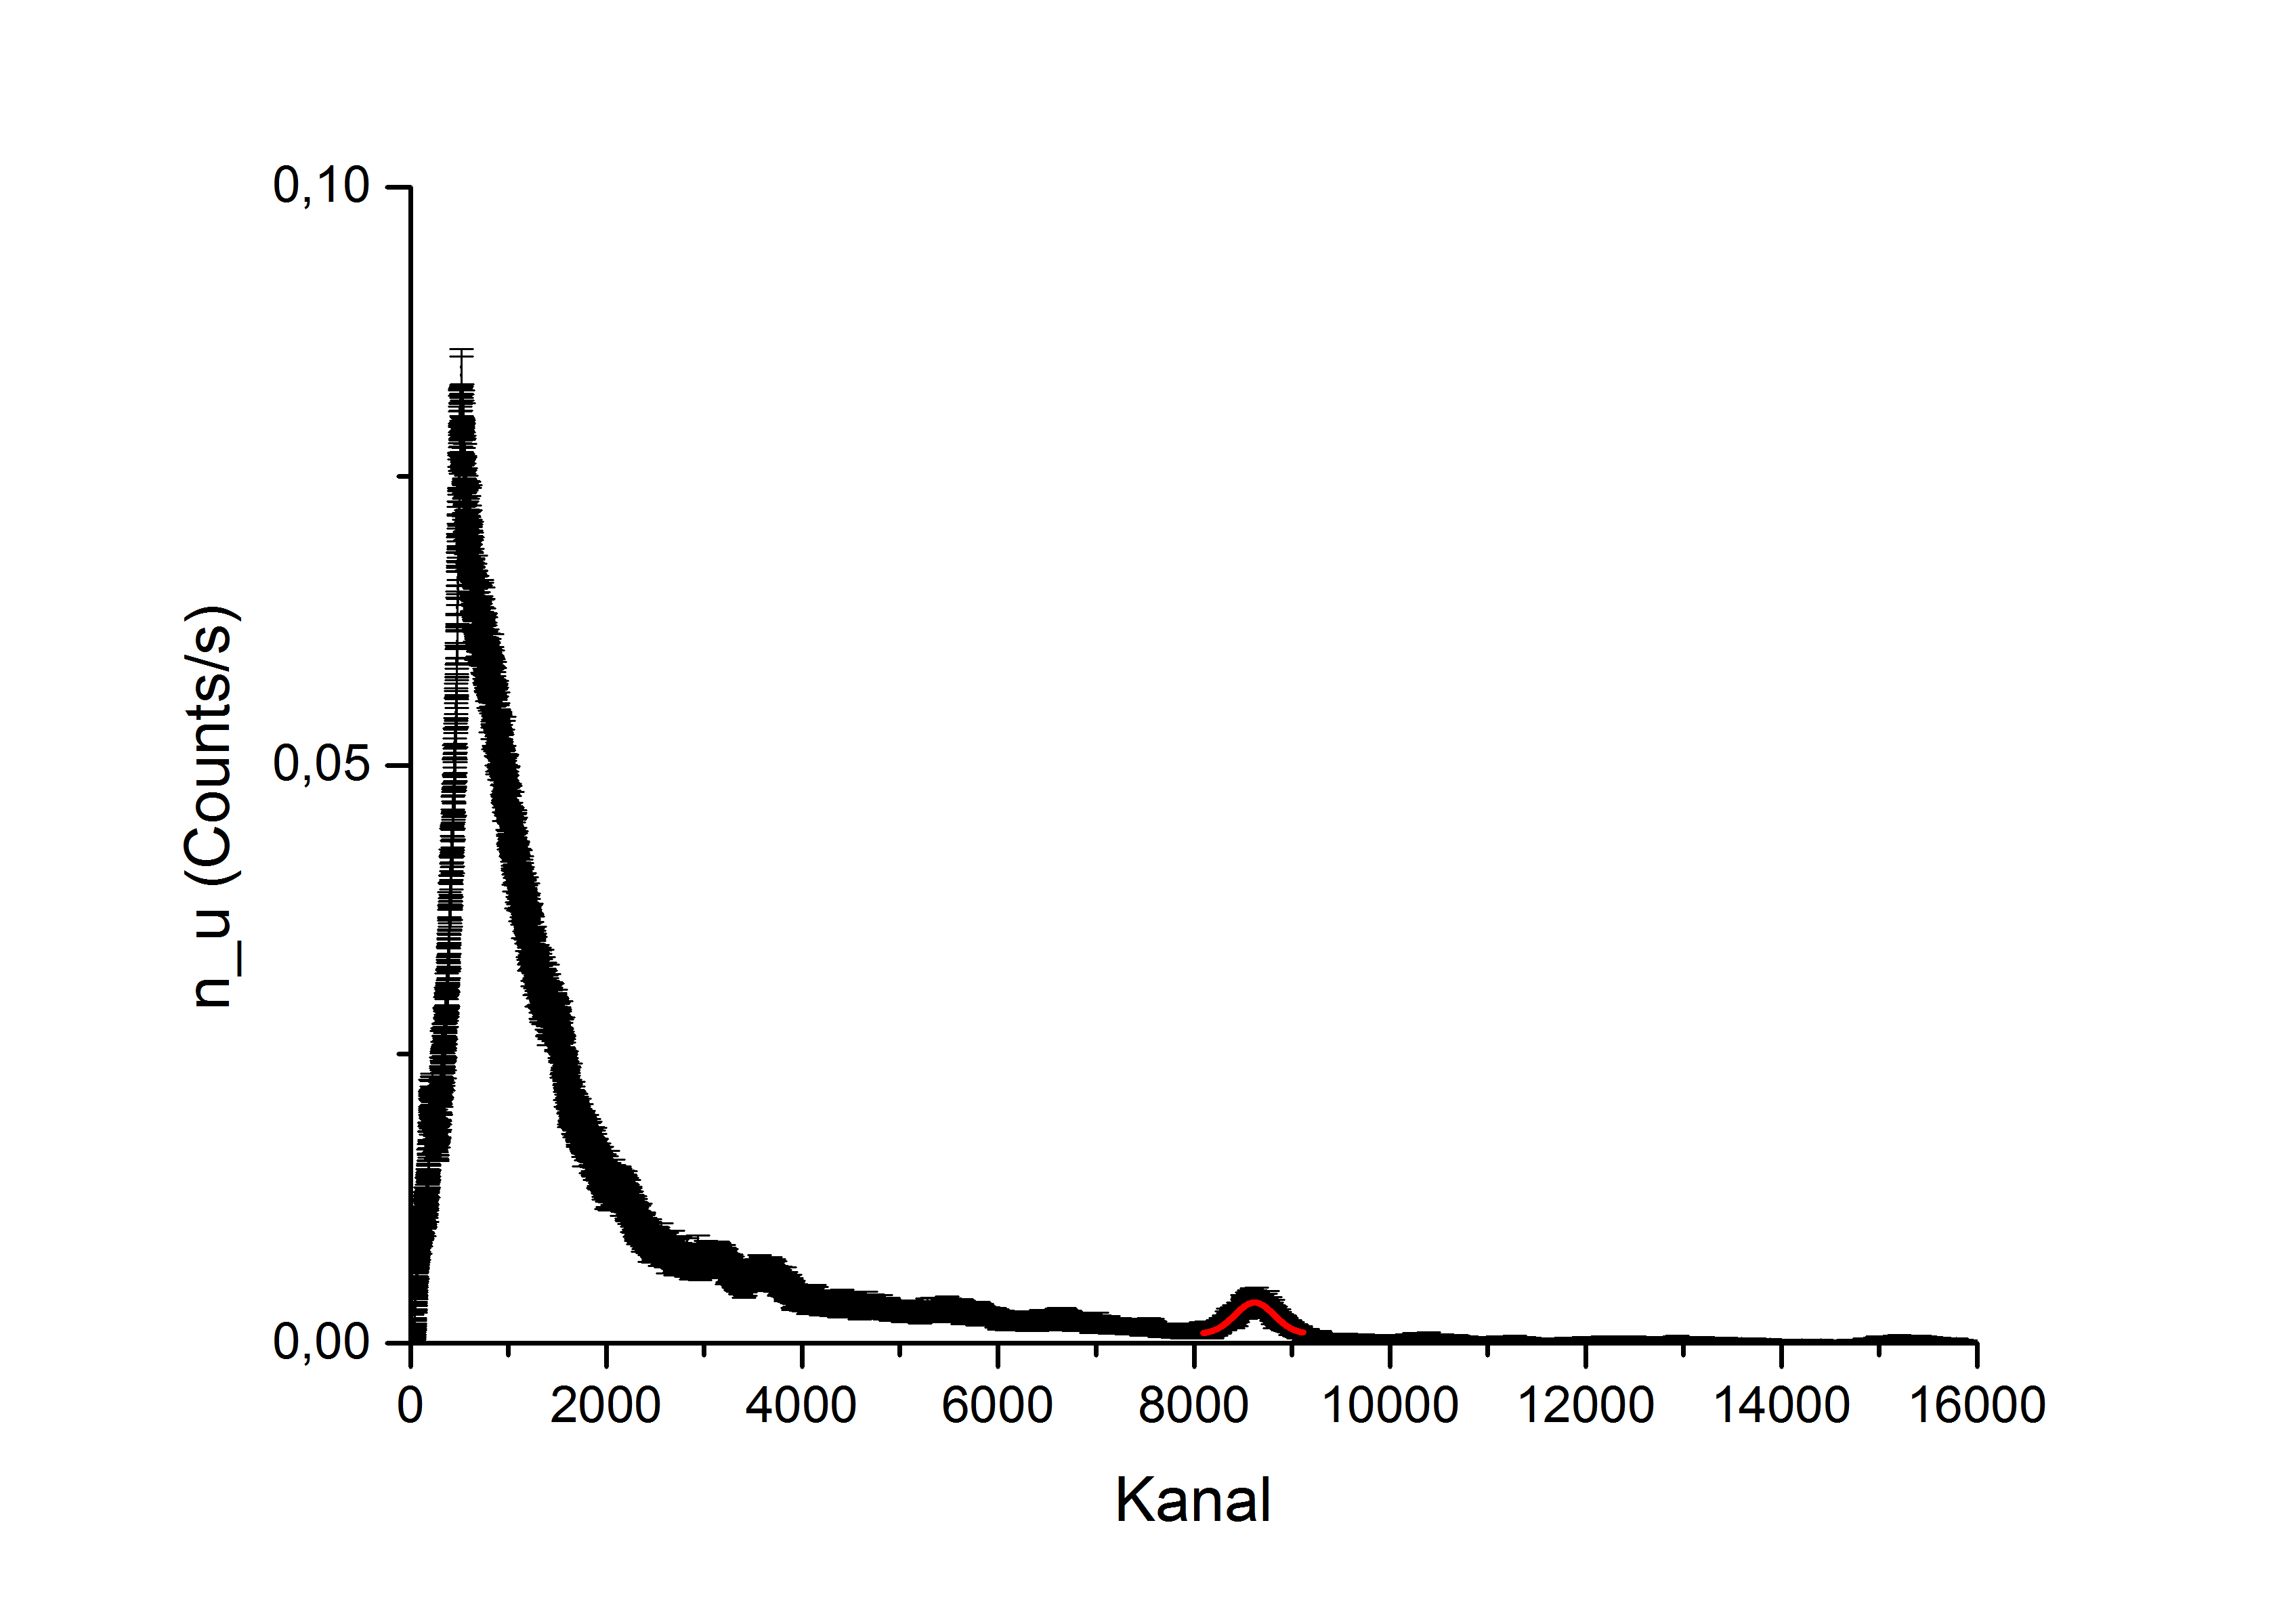
\includegraphics[scale=0.6]{Bilder/ugrund}
 \caption{Untergrundzählraten}
 \end{center}
 \end{figure}
 ~\\
 Dabei ist bei Kanal klar ein Peak zu erkennen, auf welchen wir später, nach der Energieeichung, noch zurückkommen werden.
 \subsection{Energieeichung}
 Um eine Energieeichung durchführen zu können, wurden die Spektren von $^{22}Na$, $^{60}Co$ und $^{152}Eu$ vermessen. Das charakteristische Energiespektrum dieser Proben ist bekannt, weshalb sie zur Energieeichung des MCA verwendet werden können. Die Messdauern ('Live times') t betrugen dabei $t_{^{22}Na}=917 s$, $t_{^{60}Co}=1964 s$ und $t_{^{152}Eu}=974 s$. Die Zählraten n' und deren Fehler wurden wie für den Untergrund berechnet. Die resultierenden, untergrundbereinigten Zählraten berechnen sich somit zu \[n(C)=n'(C)-n_{u}(C).\] Der Fehler ergibt sich mit Gauss'scher Fehlerfortpflanzung dann zu 
 \[s_{n}=\sqrt{s_{n'}^{2}+s_{n_{u}}^{2}}.\]
 An die Peaks der Verläufe (für $^{152}Eu$ die zwei intensivsten) wurden Gausskurven der Form 
 \[n(C)=y_{0}+A\cdot e^{-0,5(\frac{C-C_{peak}}{w})^{2}}\]
  gefittet: $C_{peak}$ gibt dabei die Position des Maximums an, w die Standardabweichung. \\
  Die Verläufe mitsamt Fits sind dem Anhang zu entnehmen. \\
  Die den aus [sta] entnommenen Energien mithilfe der Fits zugeordneten Kanäle sind folgender Tabelle zu entnehmen:\\
  \begin{table}[htbp]
  \begin{center}
  \caption{}
  \begin{tabular}{|l|l|r|r|r|}
  \hline
  Element & Kanal $C_{peak}$ & \multicolumn{1}{l|}{$\chi^2$/ndof} & \multicolumn{1}{l|}{Adj. $R^2$} & \multicolumn{1}{l|}{Energie in MeV} \\ \hline
  Na-22 & $3120,7\pm0,3$ & 1,97382 & 0,99157 & 0,511 \\ \hline
   & $7543,0\pm1,2$ & 1,02699 & 0,94316 & 1,275 \\ \hline
  Co-60 & $6942,4\pm1,3$ & 223,04646 & 0,92491 & 1,1732 \\ \hline
   & $7861,6\pm1,5$ & 303,87958 & 0,89757 & 1,3325 \\ \hline
  Eu-152 & $806,0\pm0,2$ & 1,8001 & 0,98394 & 0,122 \\ \hline
   & $2133,1\pm0,4$ & 1,23459 & 0,97889 & 0,344 \\ \hline
  \end{tabular}
  \label{}
  \end{center}
  \end{table}
  Jedem Kanal ist eine natürliche Zahl zugeordnet. Um die Genauigkeit der Eichung zu erhöhen, haben wir aber die genauen Werte, welche wir mithilfe des Gauss-Fits erhielten, verwendet. \\
  Es ist klar zu sehen, dass die Fits für $^{22}Na$ und $^{152}Eu$ sehr gut sind: Dafür sprechen die Werte für $\chi^{2}/ndof$ ($\chi^{2}$/(Anzahl der Freiheitsgrade) - englisch 'number of degrees of freedom' (ndof)), welche allesamt in der Größenordnung von 1 liegen, sowie die Werte für das korrigierte Bestimmtheitsmaß (engl. 'Adjusted $R^{2}$), welche, wenn der Fit die Messwerte perfekt beschreibt, bei 1 liegt und hier sehr nah an diesem Wert liegen.\\
  Für $^{60}Co$ sind die Fits etwas schlechter, da die Zählraten deutlich niedriger (Faktor 10 und mehr) sind als für Europium und Natrium, weshalb eine deutlich längere Messung vonnöten gewesen wäre, um ein genaueres Ergebnis zu erzielen. Wir wählten zwar die doppelte Messdauer als für die anderen beiden Materialien, jedoch ist die Genauigkeit aufgrund einer geringeren Countzahl auch so niedriger. Dennoch sind die Werte für das korrigierte Bestimmtheitsmaß ziemlich hoch und die Peaks auch optisch klar zu erkennen (s. Anhang), weshalb das Ergebnis akzeptabel ist.
\clearpage
  Mithilfe der so ermittelten Werte wurde die Energie E über die zugeordneten Kanäle $C_{peak}$ aufgetragen und ein linearer Fit der Form $E(C)=a+b*C$ gemacht, um eine Umrechnungsmöglichkeit zwischen Kanälen und Energie zu finden.
  \begin{figure}[h]
  \begin{center}
  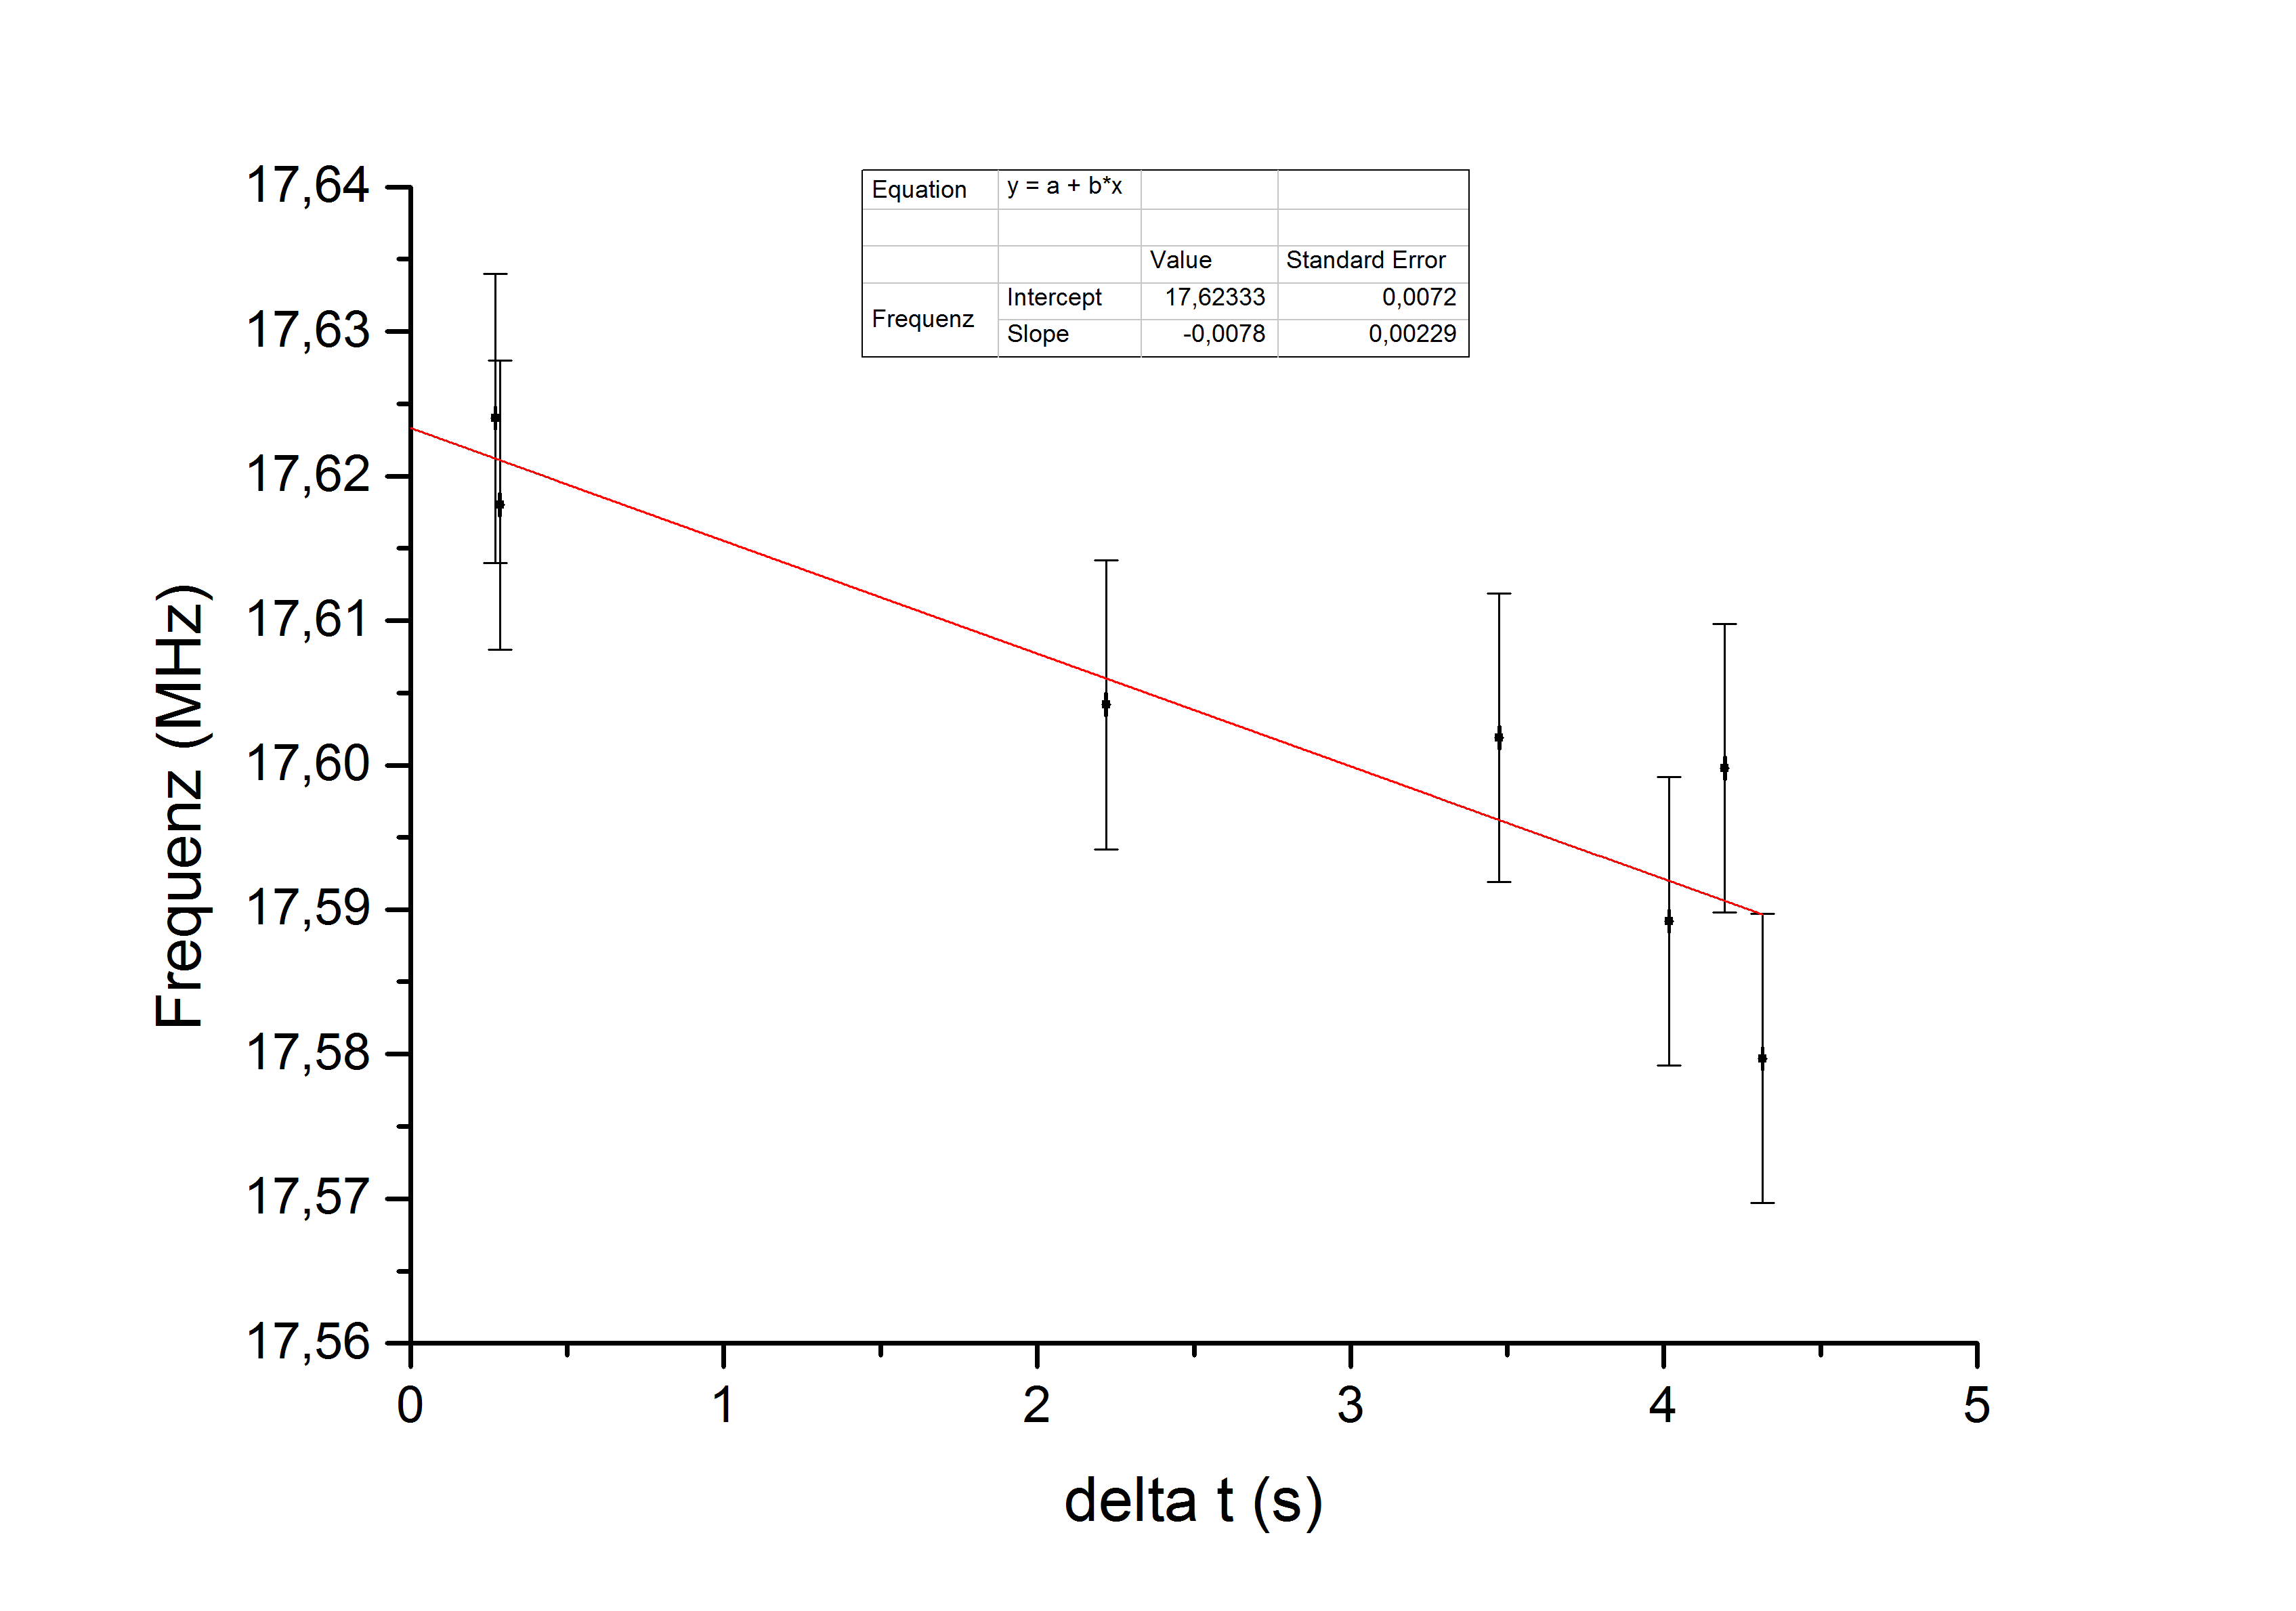
\includegraphics[scale=0.6]{Bilder/linfit}
  \caption{Linearer Fit}
  \end{center}
  \end{figure}
  Das korrigierte Bestimmtheitsmaß ('Adj. $R^{2}$) beträgt 0,99996 und ist damit sehr nahe an 1, woraus wir schließen können, dass die Daten - wie erwartet - sehr gut von einem linearen Fit beschrieben werden können. \\
  Als Umrechnungsformel von den Kanälen auf die Energie erhalten wir 
  \[E(C)=(0,1719\pm0,0005)\frac{keV}{Kanal}\cdot C+(-21\pm3)keV.\]
  Dabei ist ein Offset zu beobachten, welcher allerdings sehr gering ist.
  \subsubsection{Peak im Untergrundverlauf}
  Wie bereits erwähnt, konnte in der Untergrundmessung ein Peak beobachtet werden. Dieser wurde mit einer Gausskurve gefittet. Damit ergab sich:\\
  Kanal: $(8617,9\pm1,5)$,\\
  $\chi^{2}$/ndof=1,11715,\\
  Adj. $R^{2}$=0,92012.\\
  Der niedrige Wert für $\chi^{2}/ndof$ und besonders der ziemlich hohe Wert für das korrigierte Bestimmtheitsmaß zeugen von einem guten Fit. \\
  Mithilfe der eben berechneten Umrechnungsmethode kann die Energie des Untergrundpeaks nun berechnet werden, wobei sich der Fehler mit Gauss'scher Fehlerfortpflanzung zu 
  \[s_{E}=\sqrt{C^{2}s_{b}^{2}+s_{a}^{2}+b^{2}s_{C}^{2}}\] 
  berechnet. Somit ergibt sich als Energie des Peaks im Untergrund $E=(1461\pm5)keV$. Dabei handelt es sich vermutlich um den Zerfall von natürlich vorkommenden $^{40}K$, welches unter Anderem in den angeregten Zustand von $^{40}Ar$ zerfällt. Bei der Abregung wird ein $\gamma$-Quant mit der Energie von 1461 keV (Quelle: [sta]) freigesetzt. Die Energie des Peaks im Untergrundspektrum entspricht dieser im Rahmen der Messungenauigkeit, was die Vermutung nahelegt. 
  \clearpage
  \subsection{Analyse des $^{228}Th$-Spektrums}
  Für $^{228}Th$ betrug die tatsächliche Messdauer ('Live time') $t_{^{228}Th}=5744 s$. Die resultierende Zählrate und deren Fehler wurde analog zu dem vorherigen Unterkapitel berechnet. Die Zählrate wurde über die Kanäle aufgetragen und Peaks mithilfe der bereits diskutierten Gaussfunktion 
  \[n(C)=y_{0}+A\cdot e^{-0,5(\frac{C-C_{peak}}{w})^{2}}\]
   gefittet. Dabei haben wir aufgrund der unterschiedlichen Amplituden der Peaks das Diagramm in vier Teile aufgespalten, um diese besser sichtbar zu machen.
  \begin{figure}[h]
  \begin{center}
  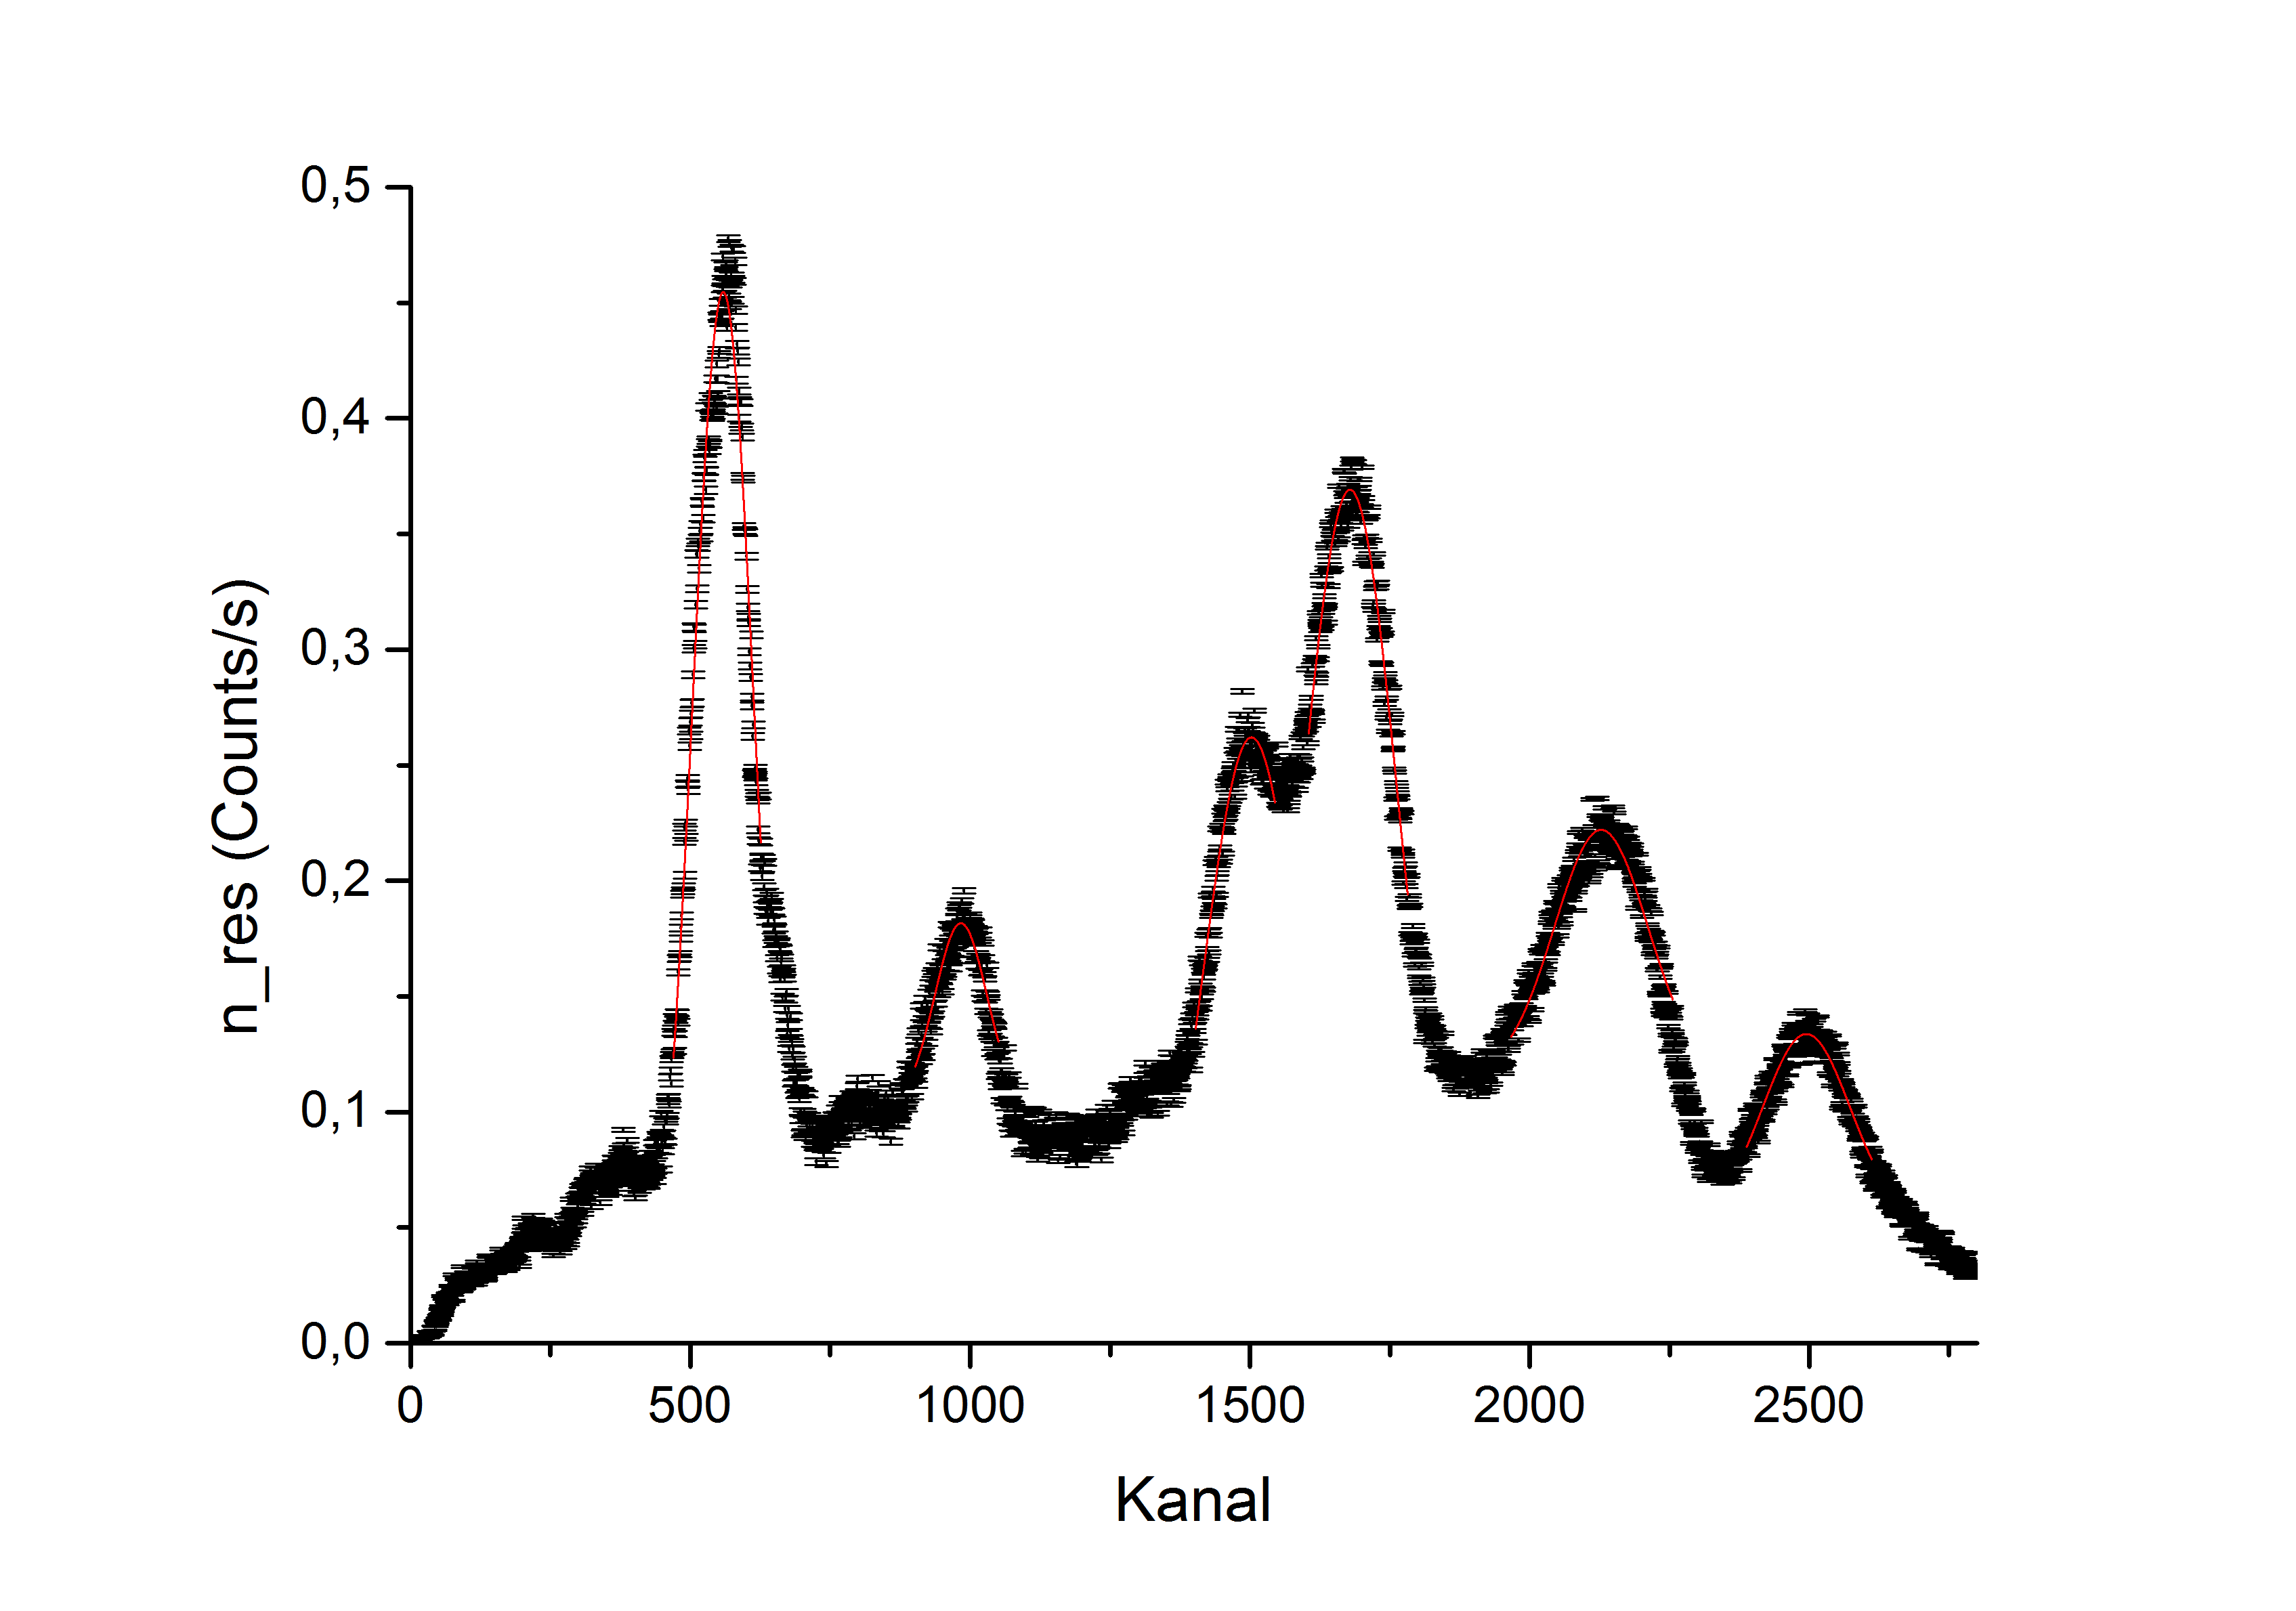
\includegraphics[scale=0.6]{Bilder/peaks1}
  \caption{Erster Teil des Thoriumspektrums}
  \end{center}
  \end{figure}
  \begin{figure}[h]
    \begin{center}
    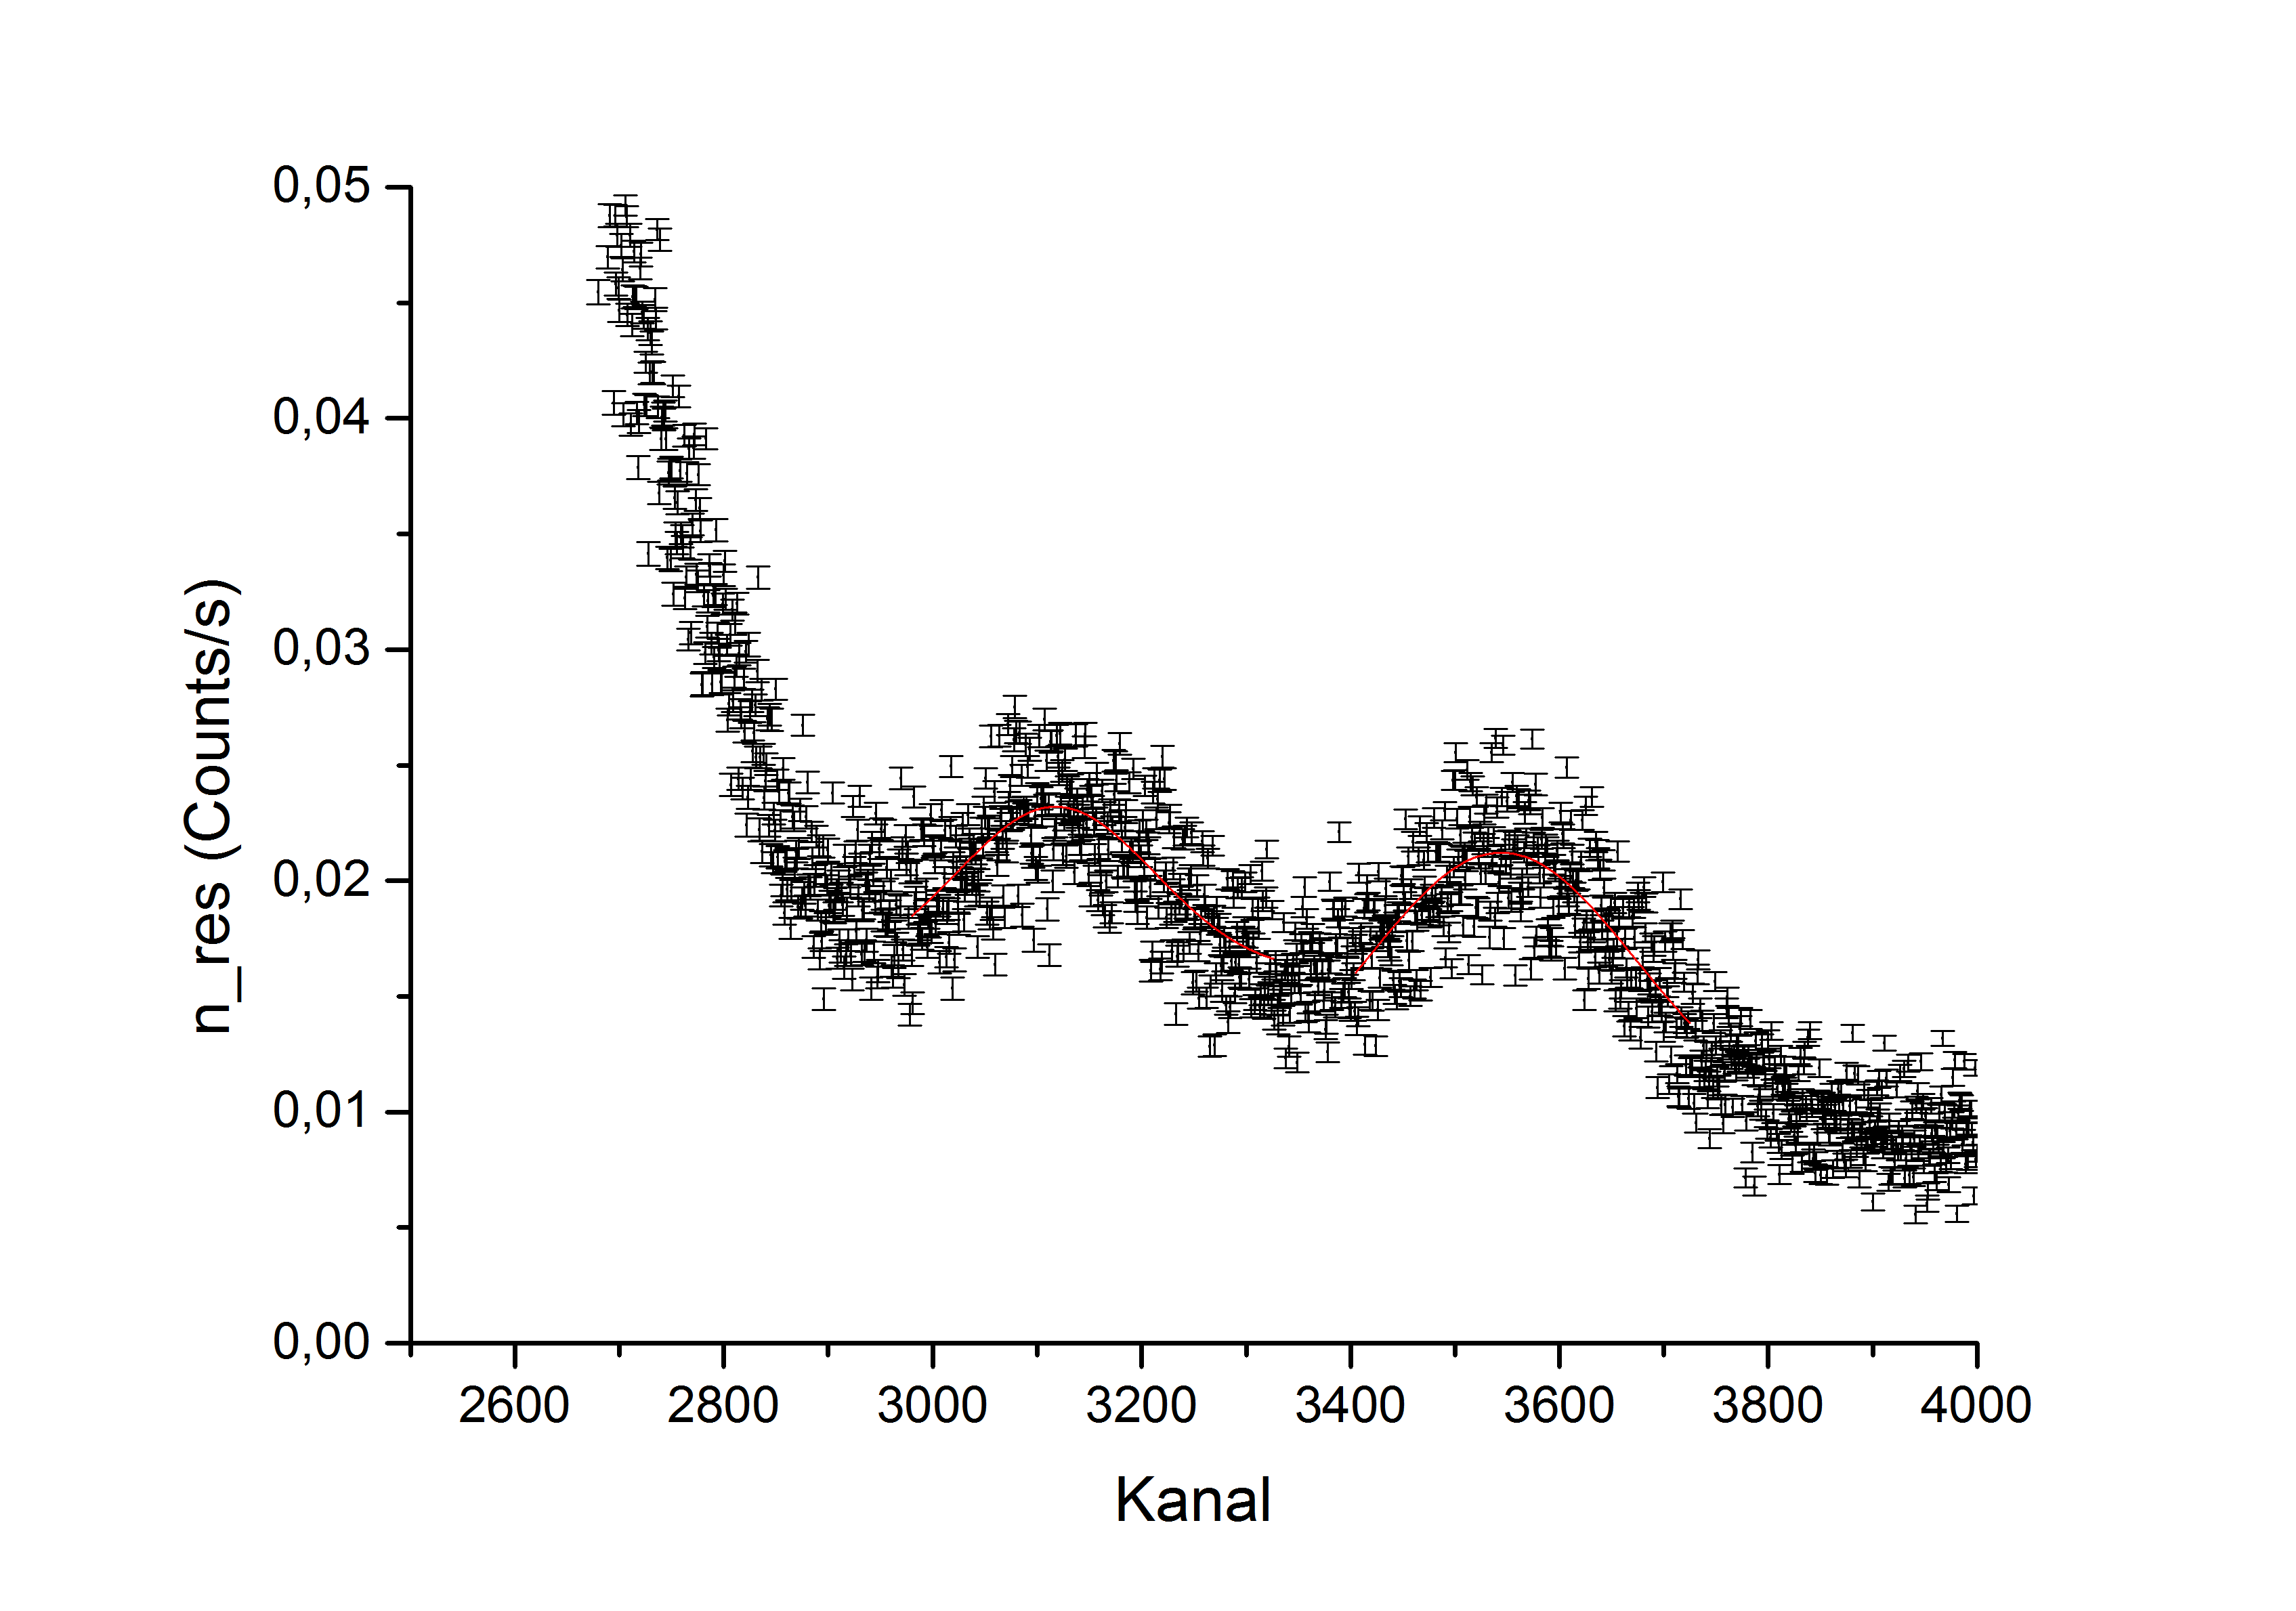
\includegraphics[scale=0.6]{Bilder/peaks2}
    \caption{Zweiter Teil des Thoriumspektrums}
    \end{center}
    \end{figure}
    \begin{figure}[h]
      \begin{center}
      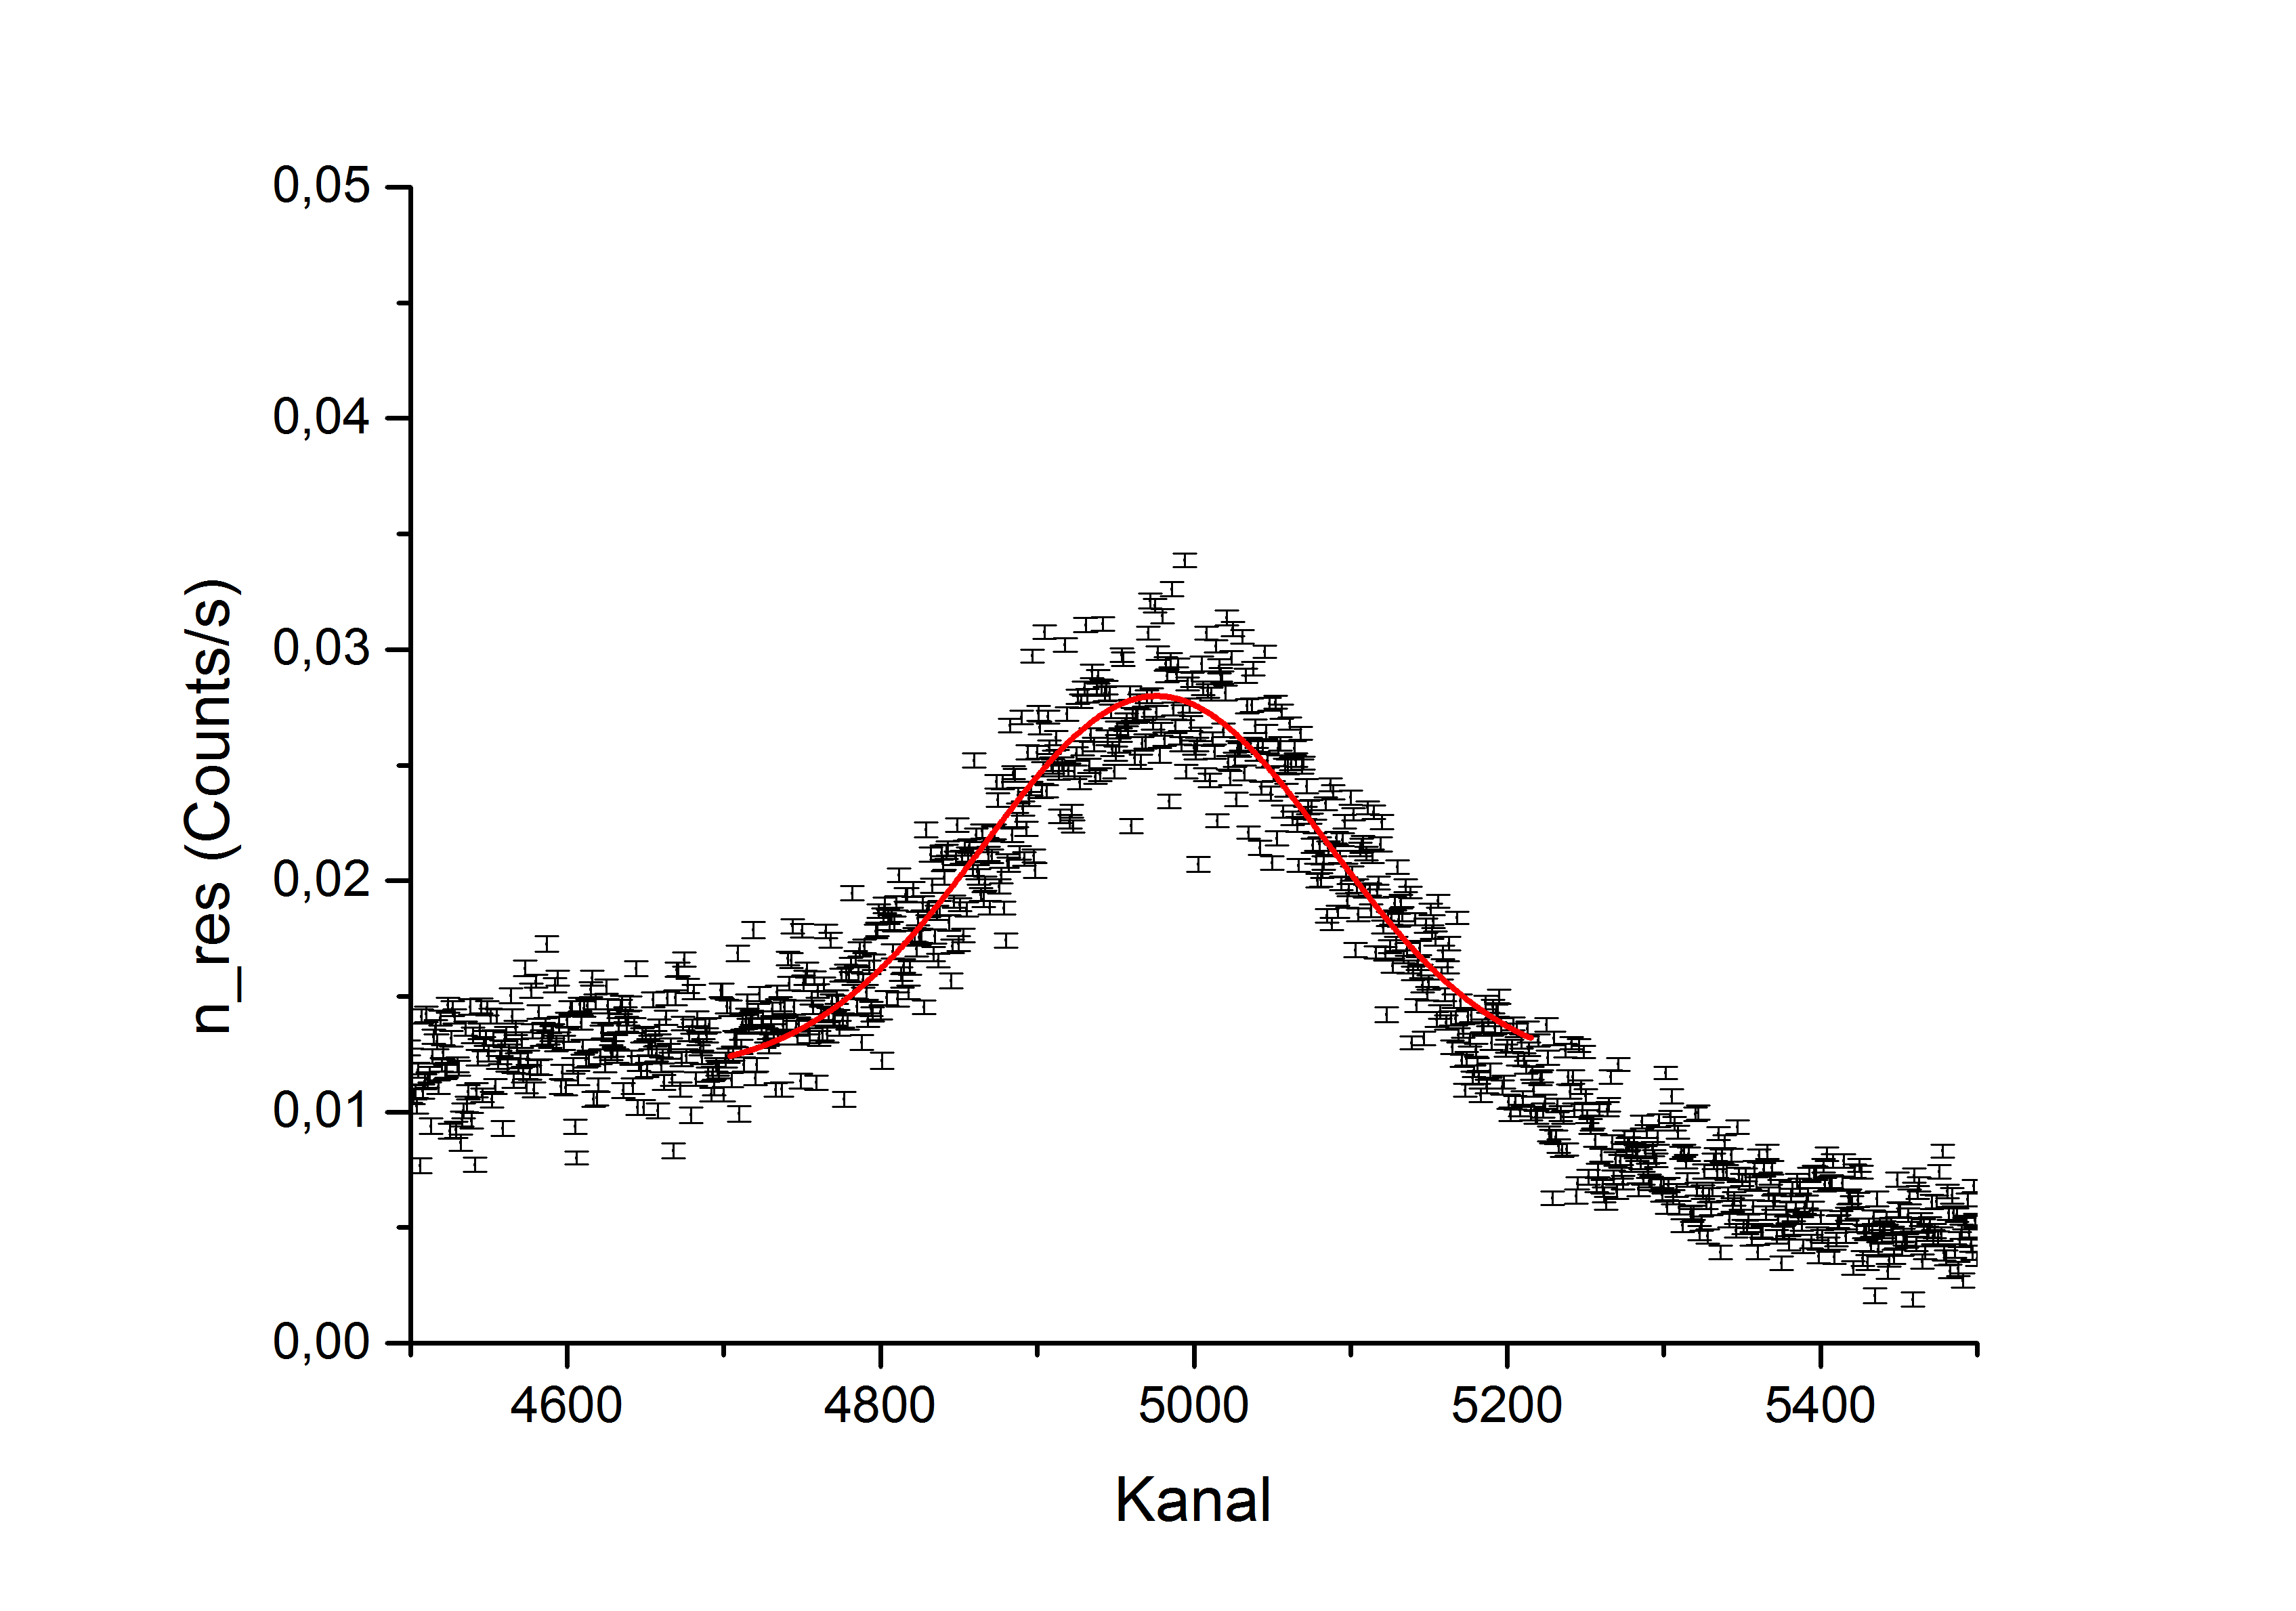
\includegraphics[scale=0.6]{Bilder/peaks4}
      \caption{Dritter Teil des Thoriumspektrums}
      \end{center}
      \end{figure}
      \begin{figure}[h]
        \begin{center}
        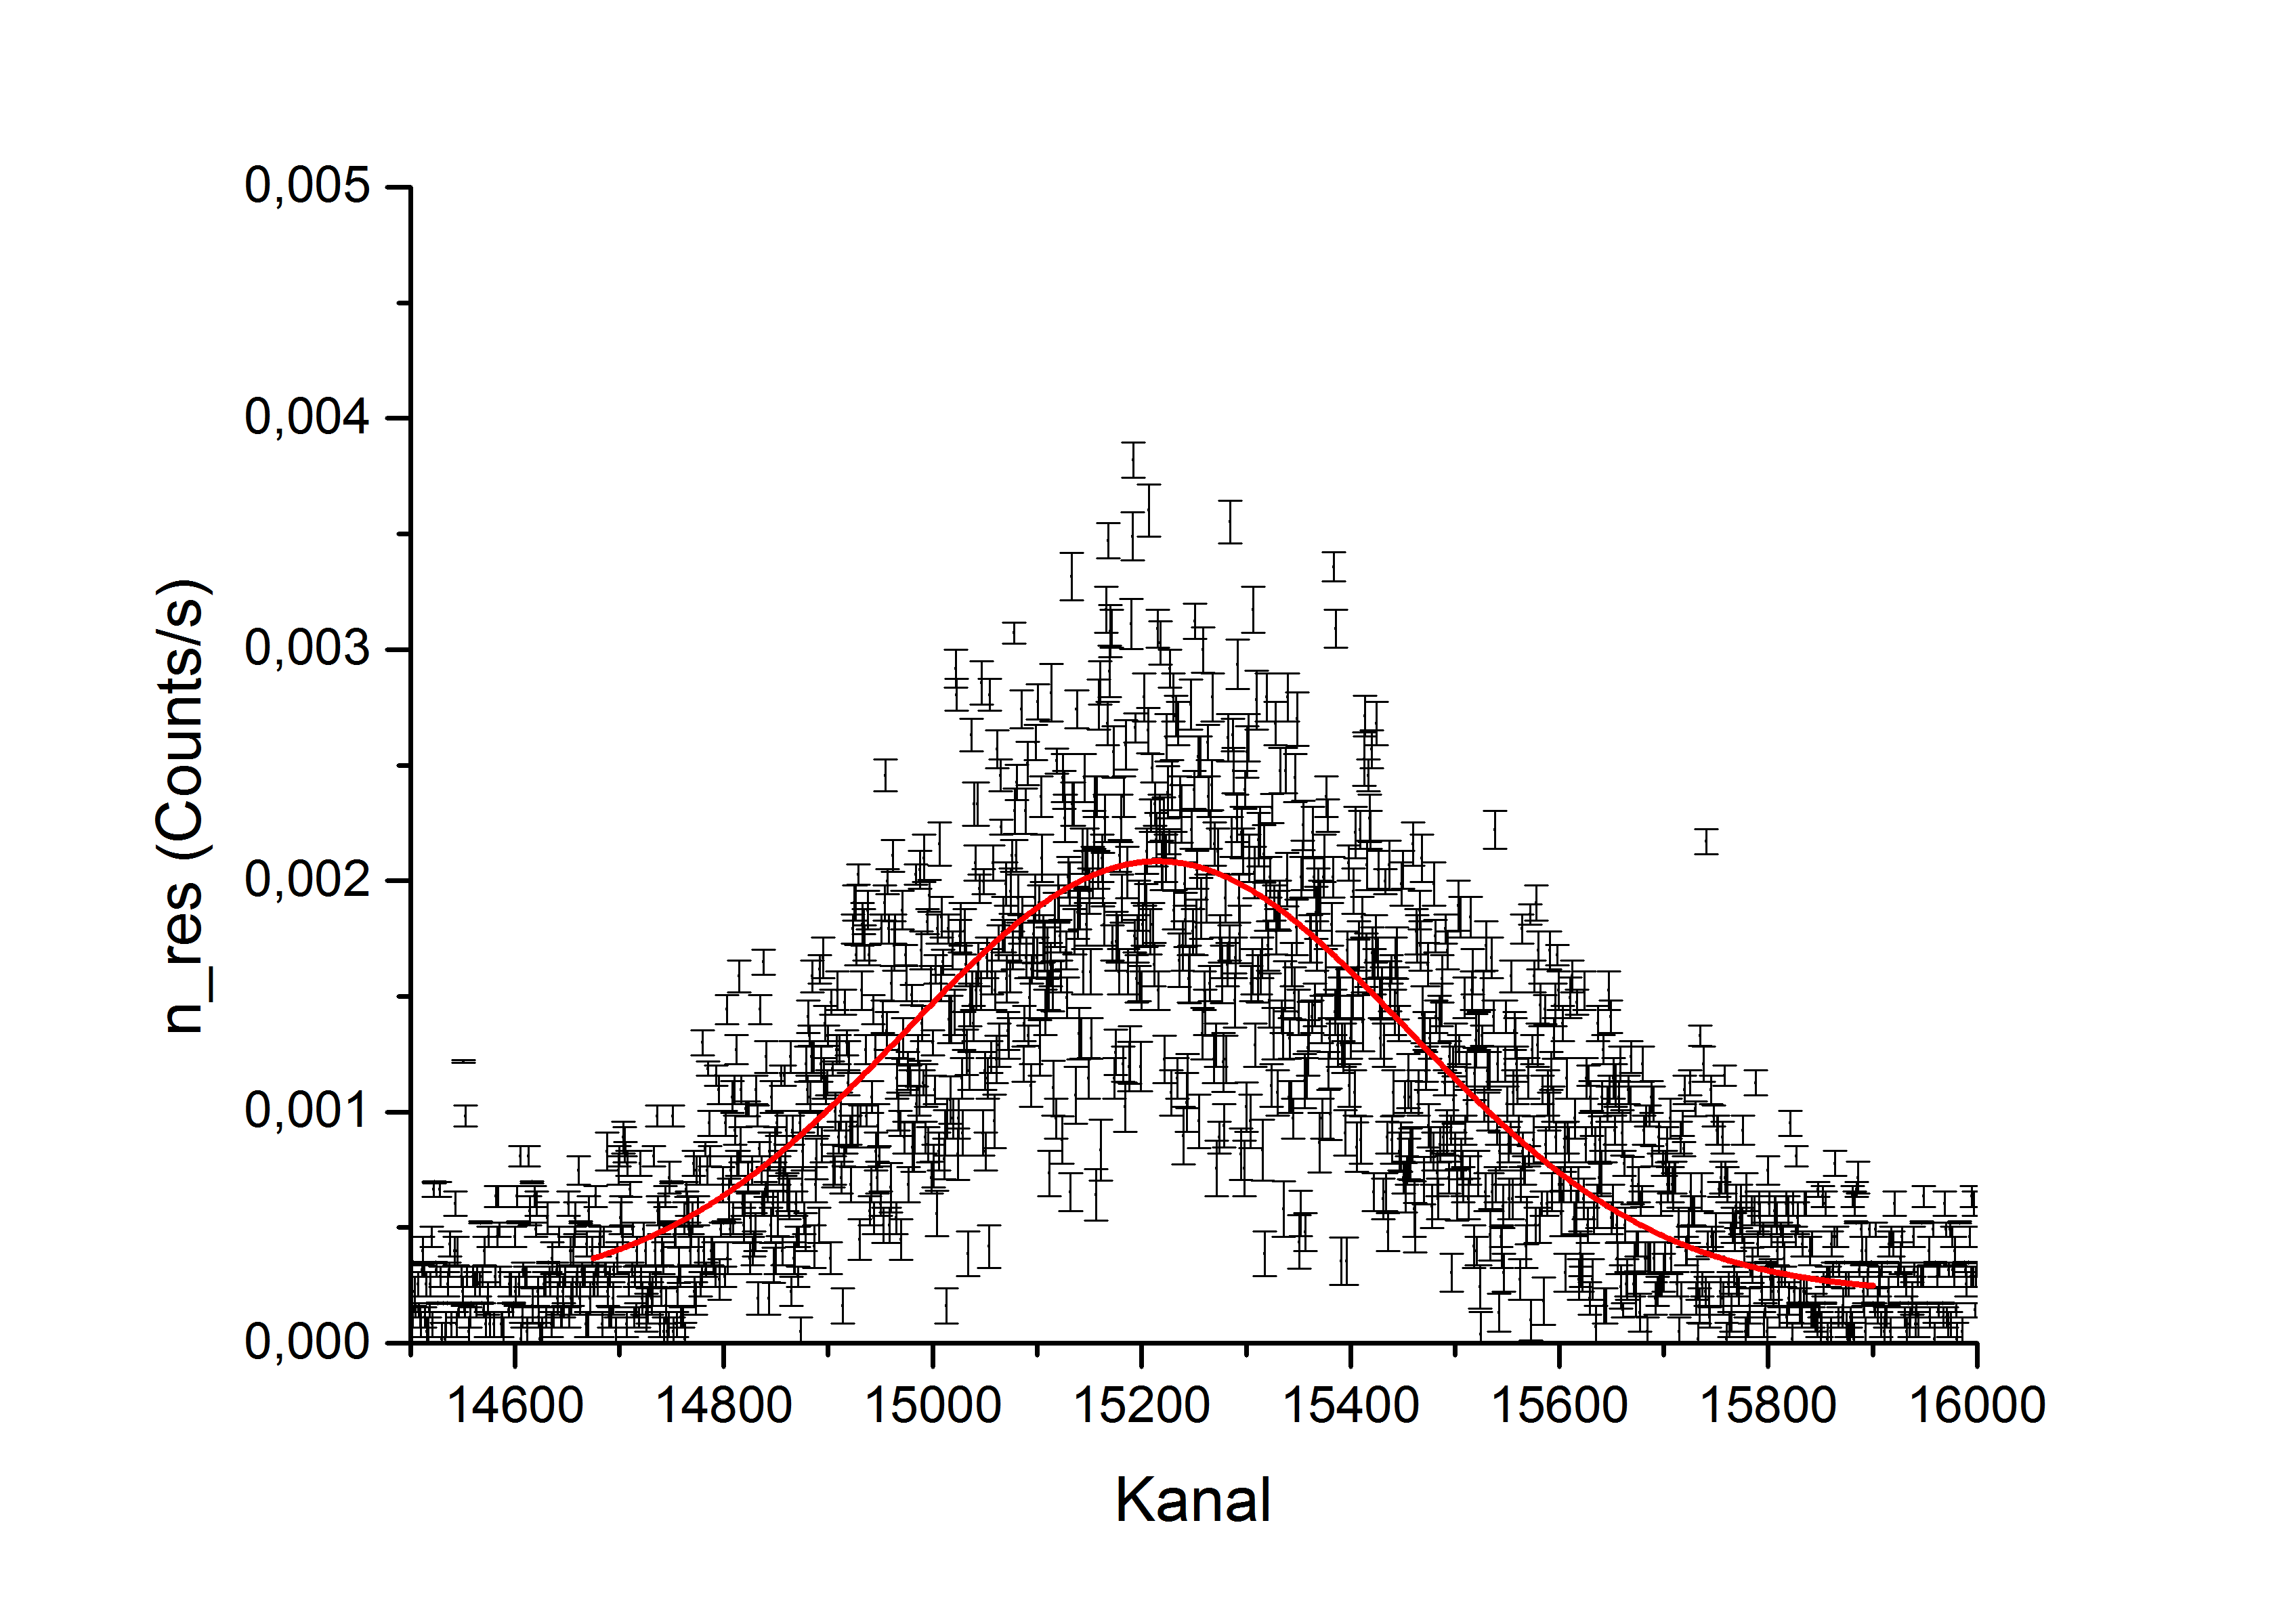
\includegraphics[scale=0.6]{Bilder/peaks3}
        \caption{Vierter Teil des Thoriumspektrums}
        \end{center}
        \end{figure}
        \clearpage
Wir erhielten 10 Peaks, für welche folgendes gilt:
\begin{table}[htbp]
\begin{center}
\caption{}
\begin{tabular}{|l|l|l|r|r|}
\hline
Kanal $C_{peak}$ & $y_{0}$ & A & \multicolumn{1}{l|}{$\chi^{2}/ndof$} & \multicolumn{1}{l|}{Adj. $R^{2}$} \\ \hline
$559,0\pm0,4$ & $0,00\pm0,03$ & $0,45\pm0,02$ & 130,44677 & 0,97255 \\ \hline
$983,8\pm0,7$ & $0,103\pm0,008$ & $0,079\pm0,008$ & 31,95607 & 0,88299 \\ \hline
$1502,9\pm0,9$ & $-0,01\pm0,05$ & $0,27\pm0,05$ & 57,0133 & 0,96581 \\ \hline
$1678,9\pm0,4$ & $0,02\pm0,04$ & $0,35\pm0,04$ & 109,08438 & 0,97422 \\ \hline
$2127,9\pm0,8$ & $0,116\pm0,005$ & $0,106\pm0,005$ & 144,6354 & 0,92679 \\ \hline
$2494,7\pm0,7$ & $0,053\pm0,008$ & $0,080\pm0,008$ & 94,91983 & 0,91688 \\ \hline
$3118\pm4$ & $0,0160\pm0,0008$ & $0,0072\pm0,0007$ & 24,06606 & 0,4671 \\ \hline
$3544\pm3$ & $0,009\pm0,004$ & $0,012\pm0,004$ & 27,91625 & 0,474 \\ \hline
$4976,3\pm1,4$ & $0,0117\pm0,0004$ & $0,0163\pm0,0004$ & 48,17991 & 0,86531 \\ \hline
$15215\pm4$ & $0,000216\pm0,000012$ & $0,00187\pm0,00004$ & 58,14617 & 0,71729 \\ \hline
\end{tabular}
\label{}
\end{center}
\end{table}
Dabei ist klar zu erkennen, dass für die hohen Peaks (bis Kanal $2494,7\pm0,7$) die Fits deutlich besser sind als für die restlichen Peaks. Die Werte für das korrigierte Bestimmtheitsmaß sind hier im Bereich von 0,9 und höher. Für die beiden Peaks bei den Kanälen $3118\pm4$ und $3544\pm3$ gilt $Adj. R^{2}<0,5$, was daran liegt, dass die Peaks räumlich sehr nahe aneinander liegen und die Zählrate niedrig ist, weshalb die Ungenauigkeiten groß werden. Die Fits für die restlichen beiden Peaks sind besser, allerdings auch nicht so gut, was daran liegt, dass die Zählrate deutlich geringer ist und damit statistische Streuungen deutlich stärker ins Gewicht fallen.\\
~\\
Auf die Peaks nehmen wir nunmehr als Peak 1-10 Bezug: Peak 1 ist dabei der Peak mit der kleinsten zugeordneten Kanalzahl, die restlichen Zahlen werden aufsteigend nach Kanalzahl zugeordnet.\\
~\\
Mithilfe der Energieeichung $E(C)=a+b\cdot C$ können nun den Peaks Energien zugeordnet werden. Diesen werden mithilfe der Zerfallsschemata in [sta] den jeweiligen verursachenden Zerfällen zugeordnet. Der Fehler auf die Energie berechnet sich mithilfe der Gauss'schen Fehlerfortpflanzung, wie bereits diskutiert, zu $s_{E}=\sqrt{s_{a}^{2}+C^{2}s_{b}^{2}+b^{2}s_{C}^{2}}$.
\clearpage
\begin{table}[h]
\begin{center}
\caption{}
\begin{tabular}{|l|l|p{10 cm}|}
\hline
 & Energie in keV & zugeordneter Zerfall (Angabe des Mutterkerns) \\ \hline
Peak 1 & $75\pm3$ & Aufgrund der hohen Intensität vermutlich Th-228 (84,4 keV). \\ \hline
Peak 2 & $148\pm3$ & Vermutlich Überlagerung der Peaks mit 131,6 keV bzw. 166,1 keV von Th-228: Getrenntes Auflösen nicht möglich. \\ \hline
Peak 3 & $237\pm3$ &  Überlagerung von Ra-224 (241,0 keV) und Pb-212 (238,6 keV) \\ \hline
Peak 4 & $268\pm3$ & Tl-208 (277,4 keV)\\ \hline
Peak 5 & $345\pm3$ & Eventuell Pb-212 (300,1 keV).  \\ \hline
Peak 6 & $408\pm3$ & Möglicherweise Bi-212 (453,0 keV). Systematische Verschiebung zu kleineren Energien durch Asymmetrie bedingt durch höheren Peak 5 möglich. \\ \hline
Peak 7 & $515\pm3$ & Tl-208 (510,8 keV). \\ \hline
Peak 8 & $588\pm3$ & Tl-208 (583,2 keV). \\ \hline
Peak 9 & $835\pm4$ & Möglicherweise Po-212 (804,9  keV). \\ \hline
Peak 10 & $2595\pm8$ & Überlagerung von Tl-208 (2614,5 keV) und Po-208 (2610,0 keV) mit geringerer Intensität. \\ \hline
\end{tabular}
\end{center}
\label{}
\end{table}
Zu den Abweichungen von den Energien der zugeordneten Zerfällen könnten Effekte wie Rückstreuung beigetragen haben. Außer den Peaks 5,6 und 9 sind aber die von uns gemessenen Werte sehr nah an den Literaturwerten. 
\subsubsection{Intensitäten}
Die Intensitäten berechnen sich aus der Höhe der Peaks. Aufgrund der Formel für die Gausskurve gilt: \[I=y_{0}+A.\] 
Der Fehler auf diese Größe berechnet sich mithilfe Gauss'scher Fehlerfortpflanzung zu 
\[s_{I}=\sqrt{s_{y_{0}}^{2}+s_{A}^{2}}.\] 
Nun muss die Charakteristik des verwendeten NaJ-Kristalls beachtet werden, welche in [ver] gegeben ist, um die Werte anzupassen. Die Werte für die Photopeak-Effizienz P haben wir aus dem Graphen abgelesen, der Fehler auf diesen Wert kommt nicht nur durch den Fehler der Energie zustande, sondern wird dominiert durch unseren Ablesefehler. Die angepasste Intensität berechnet sich dann zu \[I_{res}=\frac{1}{P}\cdot I,\]
der Fehler mittels Gauss'scher Fehlerfortpflanzung zu 
\[s_{I_{res}}=\frac{I}{P}\cdot\sqrt{\left(\frac{s_{I}}{I}\right)^{2}+\left(\frac{s_{P}}{P}\right)^{2}}.\]
\clearpage
Somit erhalten wir:
\begin{table}[htbp]
\begin{center}
\caption{}
\begin{tabular}{|l|l|l|l|}
\hline
 & Intensität I in Counts/s & Effizienz P & $I_{res}$ in Counts/s \\ \hline
Peak 1 & $0,45\pm0,04$ & $1,00\pm0,01$ & $0,45\pm0,04$ \\ \hline
Peak 2 & $0,182\pm0,011$ & $0,97\pm0,02$ & $0,187\pm0,012$ \\ \hline
Peak 3 & $0,26\pm0,07$ & $0,90\pm0,02$ & $0,29\pm0,07$ \\ \hline
Peak 4 & $0,37\pm0,05$ & $0,86\pm0,02$ & $0,43\pm0,06$ \\ \hline
Peak 5 & $0,222\pm0,007$ & $0,76\pm0,02$ & $0,292\pm0,012$ \\ \hline
Peak 6 & $0,134\pm0,012$ & $0,71\pm0,02$ & $0,188\pm0,017$ \\ \hline
Peak 7 & $0,0232\pm0,0011$ & $0,59\pm0,02$ & $0,039\pm0,002$ \\ \hline
Peak 8 & $0,021\pm0,013$ & $0,56\pm0,02$ & $0,04\pm0,02$ \\ \hline
Peak 9 & $0,0280\pm0,0006$ & $0,41\pm0,02$ & $0,068\pm0,004$ \\ \hline
Peak 10 & $0,00209\pm0,00004$ & $0,14\pm0,02$ & $0,015\pm0,002$ \\ \hline
\end{tabular}
\end{center}
\label{}
\end{table}
Da in [sta] nur relative Intensitäten gegeben sind, muss nun noch eine Normierung auf 100 erfolgen: Dazu werden die resultierenden Intensitäten von Peak i, $I_{res_{i}}$, durch $I_{res_{1}}$ von Peak 1 geteilt, da diese den höchsten Wert vorweist und das Ergebnis mit 100 multipliziert. \[I_{norm_{i}}=\frac{I_{res_{i}}}{I_{res_{1}}}\cdot 100.\] 
Der Fehler wird auch einfach durch $I_{res_{1}}$ geteilt und mit 100 multipliziert. Die so erhaltenen relativen Intensitäten werden dann mit den Literaturwerten aus [sta] verglichen.
\begin{table}[htbp]
\begin{center}
\caption{}
\begin{tabular}{|l|l|r|}
\hline
 & $I_{norm}$ & \multicolumn{1}{l|}{Literaturwert} \\ \hline
Peak 1 & $100\pm8$ & 100 \\ \hline
Peak 2 & $41\pm3$ & \multicolumn{1}{l|}{10,7 bzw. 8,49} \\ \hline
Peak 3 & $64\pm16$ & \multicolumn{1}{l|}{10 bzw. 0,41} \\ \hline
Peak 4 & $94\pm13$ & 0,636 \\ \hline
Peak 5 & $64\pm3$ & 0,757 \\ \hline
Peak 6 & $41\pm4$ & 0,101 \\ \hline
Peak 7 & $8,7\pm0,5$ & 2,28 \\ \hline
Peak 8 & $8\pm5$ & 8,52 \\ \hline
Peak 9 & $15,0\pm0,8$ & 0,0002 \\ \hline
Peak 10 & $3,3\pm0,5$ & \multicolumn{1}{l|}{10 bzw. 0,26} \\ \hline
\end{tabular}
\end{center}
\label{}
\end{table}
~\\
Für diejenigen Peaks, welchen wir zwei mögliche Übergänge zuordneten, haben wir beide Literaturwerte aufgeführt, wobei der größere Wert (vor allem bei großen Unterschieden) der relevantere Wert ist, da es wahrscheinlich ist, dass der Übergang mit höherer Intensität detektiert wurde.
Es sprechen nur Peak 8 und Peak 1 im Rahmen der Messungenauigkeit mit dem jeweiligen Literaturwert überein. Da auf Peak 1 normiert wurde (da dies der höchste Peak war), ist dies allerdings ein Ergebnis unserer Vorgehensweise.\\
Für die anderen Peaks sind erhebliche Diskrepanzen zwischen errechnetem Wert und Literaturwert zu beobachten. Dies kann darauf hinweisen, dass falsche Zuordnungen aufgrund der Energien erfolgten. Es ist aber auch möglich, dass zu wenige Counts für Peak 1 und Peak 10 bzw. zu viele für die übrigen Peaks (außer Peak 8) gemessen wurden.


%Inhaltsverzeichnis
\end{document}
